%%%%%%%%%%%%%%
%% Run LaTeX on this file several times to get Table of Contents,
%% cross-references, and citations.

%% If you have font problems, you may edit the w-bookps.sty file
%% to customize the font names to match those on your system.

%% w-bksamp.tex. Current Version: Feb 16, 2012
%%%%%%%%%%%%%%%%%%%%%%%%%%%%%%%%%%%%%%%%%%%%%%%%%%%%%%%%%%%%%%%%
%
%  Sample file for
%  Wiley Book Style, Design No.: SD 001B, 7x10
%  Wiley Book Style, Design No.: SD 004B, 6x9
%
%
%  Prepared by Amy Hendrickson, TeXnology Inc.
%  http://www.texnology.com
%%%%%%%%%%%%%%%%%%%%%%%%%%%%%%%%%%%%%%%%%%%%%%%%%%%%%%%%%%%%%%%%

%%%%%%%%%%%%%
% 7x10
%\documentclass{wileySev}

% 6x9
\documentclass{wileySix}

\usepackage{graphicx}
\usepackage{gensymb}
\usepackage{listings}
\usepackage{float}

\usepackage{color}
 
\definecolor{codegreen}{rgb}{0,0.6,0}
\definecolor{codegray}{rgb}{0.5,0.5,0.5}
\definecolor{codepurple}{rgb}{0.58,0,0.82}
\definecolor{backcolour}{rgb}{0.95,0.95,0.92}
 
\lstdefinestyle{mystyle}{
    backgroundcolor=\color{backcolour},   
    commentstyle=\color{codegreen},
    keywordstyle=\color{magenta},
    numberstyle=\tiny\color{codegray},
    stringstyle=\color{codepurple},
    basicstyle=\footnotesize,
    breakatwhitespace=false,         
    breaklines=true,                 
    captionpos=b,                    
    keepspaces=true,                 
    numbers=left,                    
    numbersep=5pt,                  
    showspaces=false,                
    showstringspaces=false,
    showtabs=false,                  
    tabsize=2,
    language=sh
}
 
\lstset{style=mystyle}


%%%%%%%
%% for times math: However, this package disables bold math (!)
%% \mathbf{x} will still work, but you will not have bold math
%% in section heads or chapter titles. If you don't use math
%% in those environments, mathptmx might be a good choice.

% \usepackage{mathptmx}

% For PostScript text
\usepackage{w-bookps}

%%%%%%%%%%%%%%%%%%%%%%%%%%%%%%%%%%%%%%%%%%%%%%%%%%%%%%%%%%%%%%%%
%% Other packages you might want to use:

% for chapter bibliography made with BibTeX
% \usepackage{chapterbib}

% for multiple indices
% \usepackage{multind}

% for answers to problems
% \usepackage{answers}

%%%%%%%%%%%%%%%%%%%%%%%%%%%%%%
%% Change options here if you want:
%%
%% How many levels of section head would you like numbered?
%% 0= no section numbers, 1= section, 2= subsection, 3= subsubsection
%%==>>
\setcounter{secnumdepth}{3}

%% How many levels of section head would you like to appear in the
%% Table of Contents?
%% 0= chapter titles, 1= section titles, 2= subsection titles, 
%% 3= subsubsection titles.
%%==>>
\setcounter{tocdepth}{2}

%% Cropmarks? good for final page makeup
%% \docropmarks

%%%%%%%%%%%%%%%%%%%%%%%%%%%%%%
%
% DRAFT
%
% Uncomment to get double spacing between lines, current date and time
% printed at bottom of page.
% \draft
% (If you want to keep tables from becoming double spaced also uncomment
% this):
% \renewcommand{\arraystretch}{0.6}
%%%%%%%%%%%%%%%%%%%%%%%%%%%%%%

%%%%%%% Demo of section head containing sample macro:
%% To get a macro to expand correctly in a section head, with upper and
%% lower case math, put the definition and set the box 
%% before \begin{document}, so that when it appears in the 
%% table of contents it will also work:

\newcommand{\VT}[1]{\ensuremath{{V_{T#1}}}}

%% use a box to expand the macro before we put it into the section head:

\newbox\sectsavebox
\setbox\sectsavebox=\hbox{\boldmath\VT{xyz}}

%%%%%%%%%%%%%%%%% End Demo


\begin{document}


\booktitle{Aplikasi ActSpot (M-Absensi)}
\subtitle{Android MySQL Project}

\authors{Kadek Diva Krishna Murti \& Chandra Kirana Poetra\\
\affil{D4 Teknik Informatika, Politeknik Pos Indonesia}
%Floyd J. Fowler, Jr.\\
%\affil{University of New Mexico}
}

\offprintinfo{Aplikasi ActSpot (M-Absensi), First Edition}{Kadek Diva Krishna Murti \& Chandra Kirana Poetra}

%% Can use \\ if title, and edition are too wide, ie,
%% \offprintinfo{Survey Methodology,\\ Second Edition}{Robert M. Groves}

%%%%%%%%%%%%%%%%%%%%%%%%%%%%%%
%% 
\halftitlepage

\titlepage


\begin{copyrightpage}{2020}
%Survey Methodology / Robert M. Groves . . . [et al.].
%\       p. cm.---(Wiley series in survey methodology)
%\    ``Wiley-Interscience."
%\    Includes bibliographical references and index.
%\    ISBN 0-471-48348-6 (pbk.)
%\    1. Surveys---Methodology.  2. Social 
%\  sciences---Research---Statistical methods.  I. Groves, Robert M.  II. %
%Series.\\
%
%HA31.2.S873 2007
%001.4'33---dc22                                             2004044064
\end{copyrightpage}

\dedication{`Jika Kamu tidak dapat menahan lelahnya belajar, 
Maka kamu harus sanggup menahan perihnya Kebodohan.'
~Imam Syafi'i~}

\begin{contributors}
\name{Rolly Maulana Awangga,} Informatics Research Center., Politeknik Pos Indonesia, Bandung,
Indonesia



\end{contributors}

\contentsinbrief
\tableofcontents
\listoffigures
\listoftables
\lstlistoflistings


\begin{foreword}
Sepatah kata dari Kaprodi, Kabag Kemahasiswaan dan Mahasiswa
\end{foreword}

\begin{preface}
Buku ini diciptakan bagi yang awam dengan pemrograman Android sekalipun.

\prefaceauthor{D. K. Murti \& C. K. Poetra}
\where{Bandung, Jawa Barat\\
Januari, 2020}
\end{preface}


\begin{acknowledgments}
Terima kasih atas semua masukan dari para rekan-rekan agar bisa membuat buku ini 
lebih baik dan lebih mudah dimengerti.

Terima kasih ini juga ditujukan khusus untuk team IRC yang 
telah fokus untuk belajar dan memahami bagaimana buku ini mendampingi proses 
Proyek 3.
\authorinitials{D. K. M. \& C. K. P.}
\end{acknowledgments}

\begin{acronyms}
\acro{ACGIH}{American Conference of Governmental Industrial Hygienists}
\acro{AEC}{Atomic Energy Commission}
\acro{OSHA}{Occupational Health and Safety Commission}
\acro{SAMA}{Scientific Apparatus Makers Association}
\end{acronyms}

\begin{glossary}
\term{git}Merupakan manajemen sumber kode yang dibuat oleh linus torvald.

\term{bash}Merupakan bahasa sistem operasi berbasiskan *NIX.

\term{linux}Sistem operasi berbasis sumber kode terbuka yang dibuat oleh Linus Torvald
\end{glossary}

\begin{symbols}
\term{A}Amplitude

\term{\hbox{\&}}Propositional logic symbol 

\term{a}Filter Coefficient

\bigskip

\term{\mathcal{B}}Number of Beats
\end{symbols}

\begin{introduction}

%% optional, but if you want to list author:

\introauthor{Rolly Maulana Awangga, S.T., M.T.}
{Informatics Research Center\\
Bandung, Jawa Barat, Indonesia}

Pada era disruptif  \index{disruptif}\index{disruptif!modern} 
saat ini. git merupakan sebuah kebutuhan dalam sebuah organisasi pengembangan perangkat lunak.
Buku ini diharapkan bisa menjadi penghantar para programmer, analis, IT Operation dan Project Manajer.
Dalam melakukan implementasi git pada diri dan organisasinya.

Rumusnya cuman sebagai contoh aja biar keren\cite{awangga2018sampeu}.

\begin{equation}
ABC {\cal DEF} \alpha\beta\Gamma\Delta\sum^{abc}_{def}
\end{equation}

\end{introduction}

%%%%%%%%%%%%%%%%%%Isi Buku_

%%\chapter{Persiapan}
%%\section{Persiapan dan pengenalan}
\subsection{Instalasi Java}
\subsection{Instalasi Android Studio}
\begin{enumerate}
	\item Kemudian klik dua kali pada installer yang telah di-download untuk memulai proses instalasi. Installer akan menampilkan Android Studio Setup seperti gambar berikut, lalu klik Next. 
	\begin{figure}[H]
		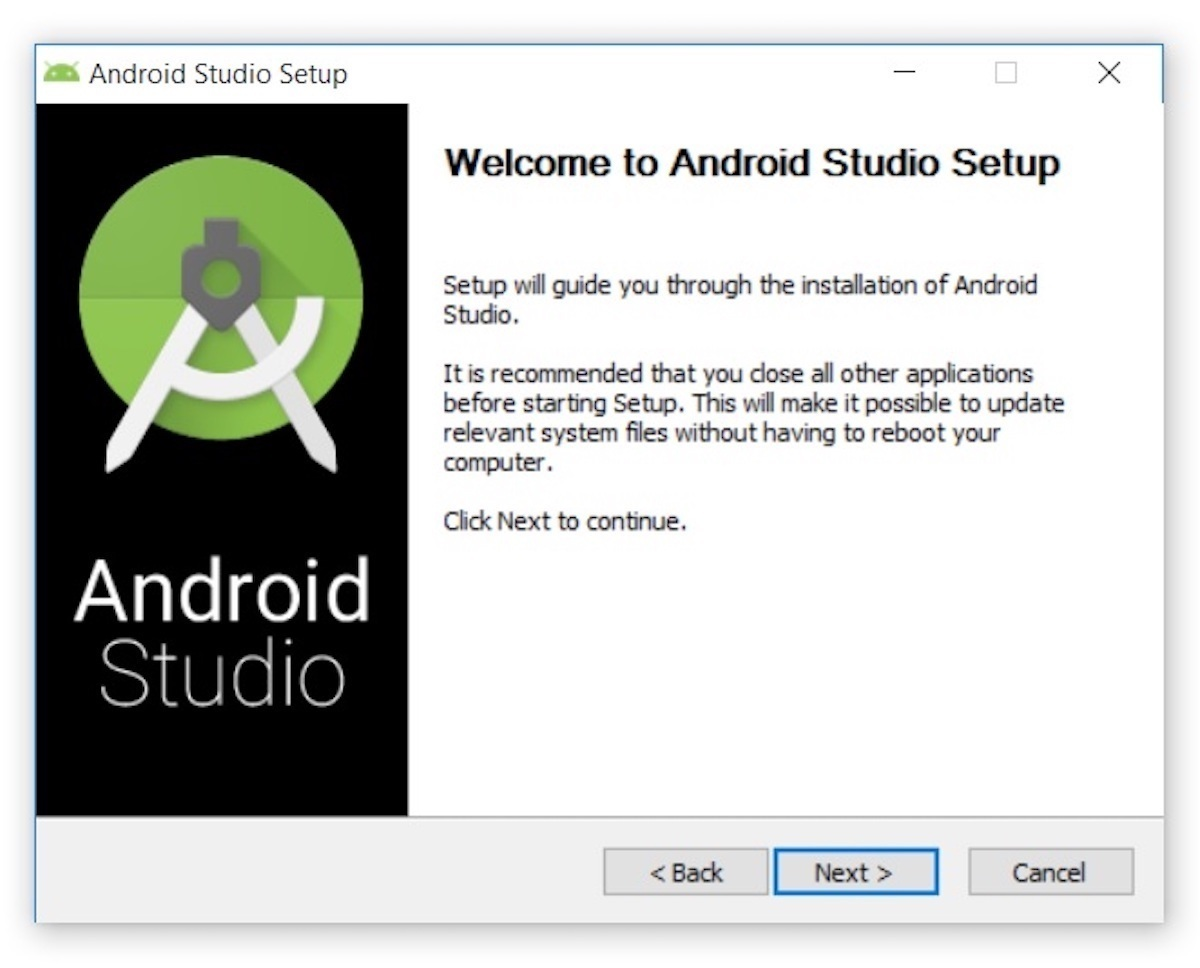
\includegraphics[width=4cm]{figures/installas/1.jpg}
		\centering
		\caption{Android Studio Setup.}
	\end{figure}
	\item Setelah itu kita diberi opsi untuk menginstal Android Virtual Device. Disini kita biarkan default setting-nya, lalu klik Next.
	\begin{figure}[H]
		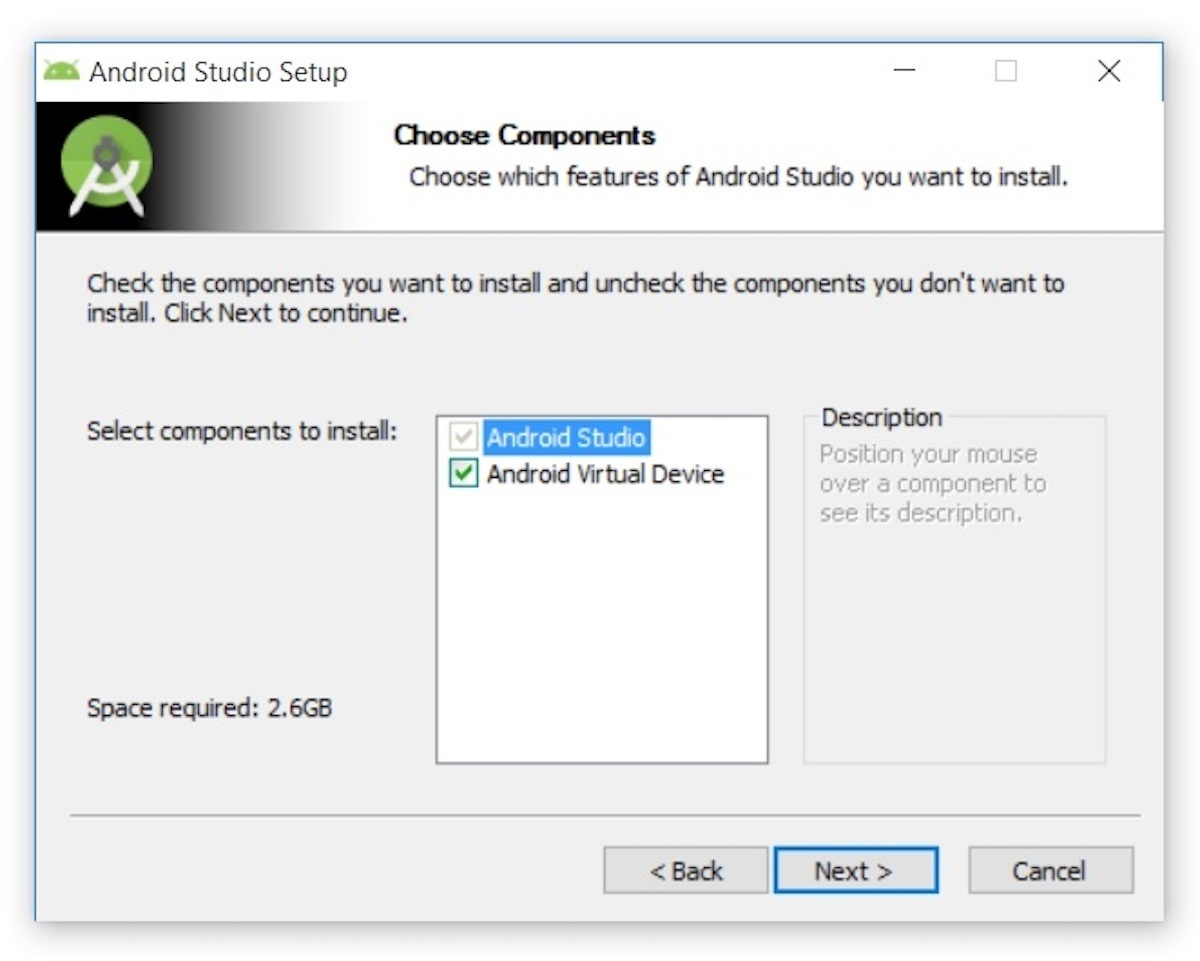
\includegraphics[width=4cm]{figures/installas/2.jpg}
		\centering
		\caption{Instal Android AVD.}
	\end{figure}
	\item Kemudian kita diminta untuk memilih lokasi tempat menginstal Android Studio-nya. Disini kita biarkan default setting-nya, lalu klik Next.
	\begin{figure}[H]
		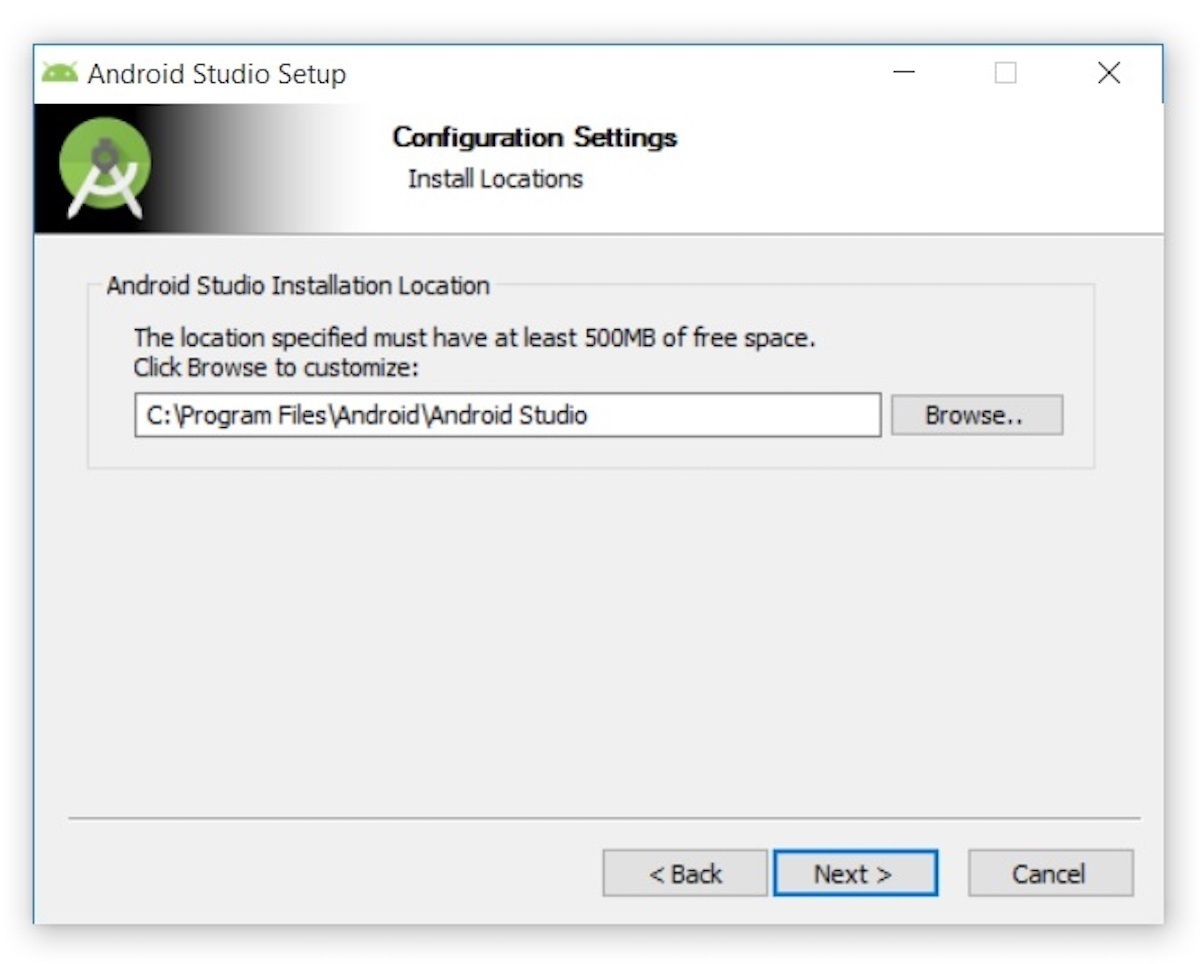
\includegraphics[width=4cm]{figures/installas/3.jpg}
		\centering
		\caption{Lokasi instal Android Studio.}
	\end{figure}
	\item Setelah itu, kita diberi opsi untuk membuat shortcut dari Android Studio. Disini kita biarkan default setting-nya, lalu klik Install.
	\begin{figure}[H]
		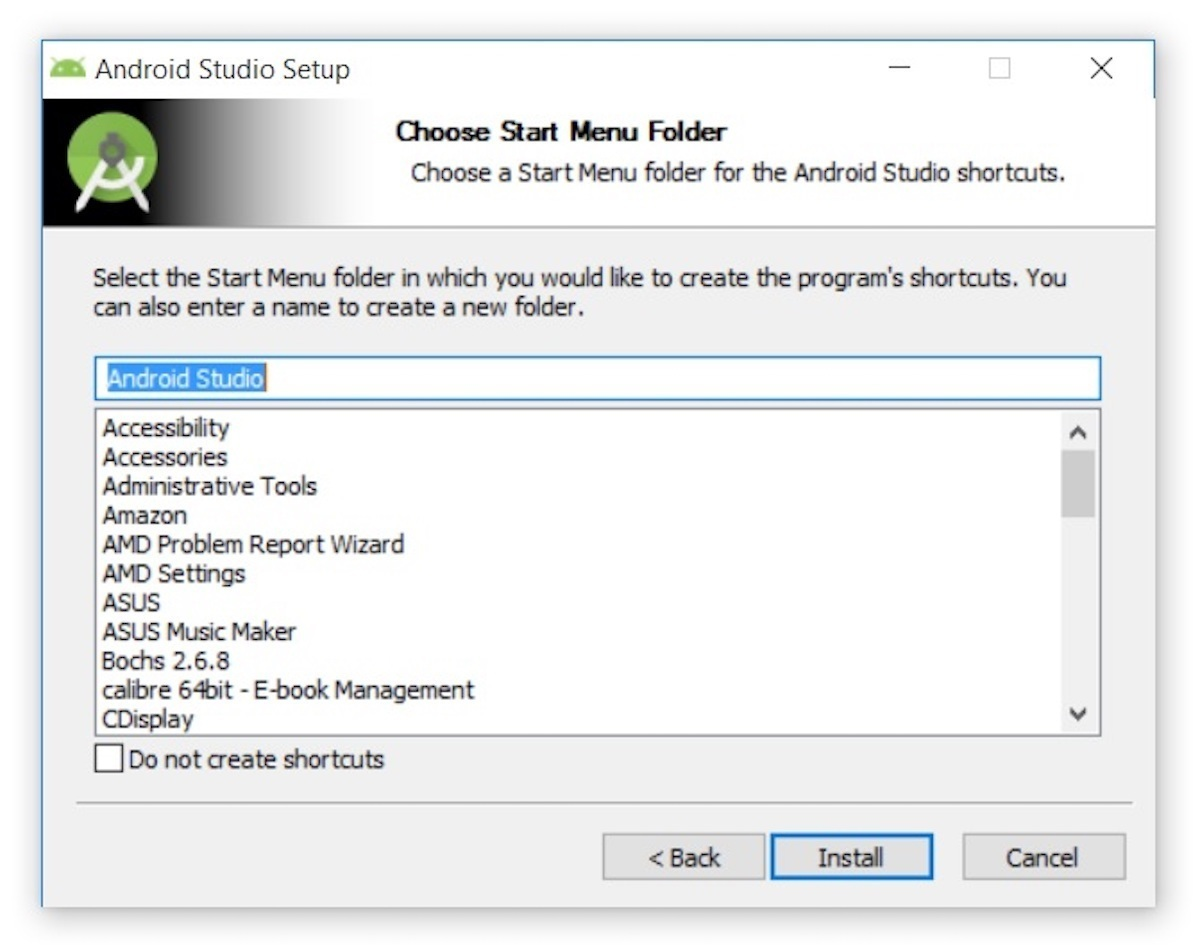
\includegraphics[width=4cm]{figures/installas/4.jpg}
		\centering
		\caption{Membuat shorcut Android Studio.}
	\end{figure}
	\item Kemudian proses instalasi akan berjalan. Show details untuk menampilkan file yang diinstal.
	\begin{figure}[h!]
		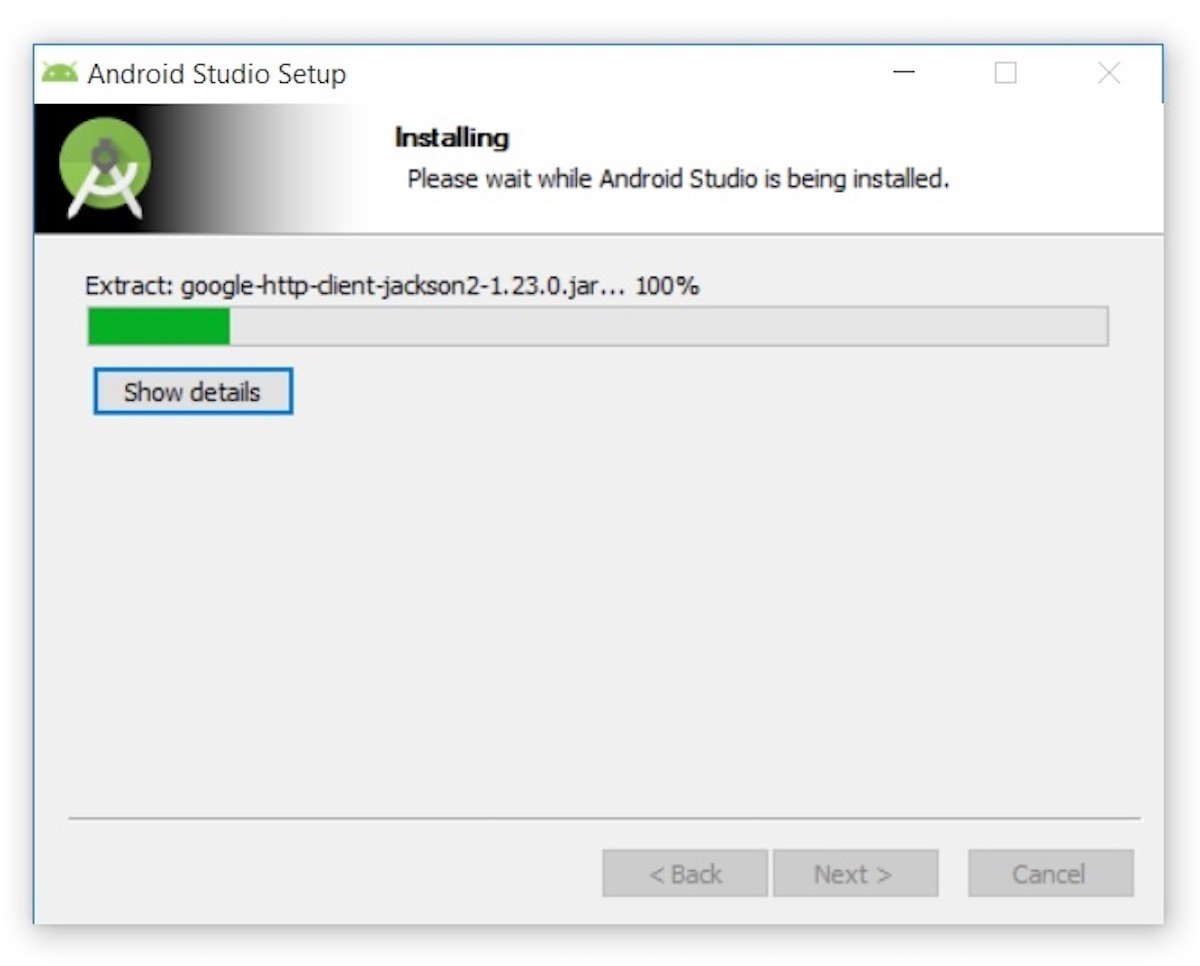
\includegraphics[width=4cm]{figures/installas/5.jpg}
		\centering
		\caption{Proses instalasi.}
	\end{figure}
	\item Setelah proses instal selesai, klik Next.
	\begin{figure}[H]
		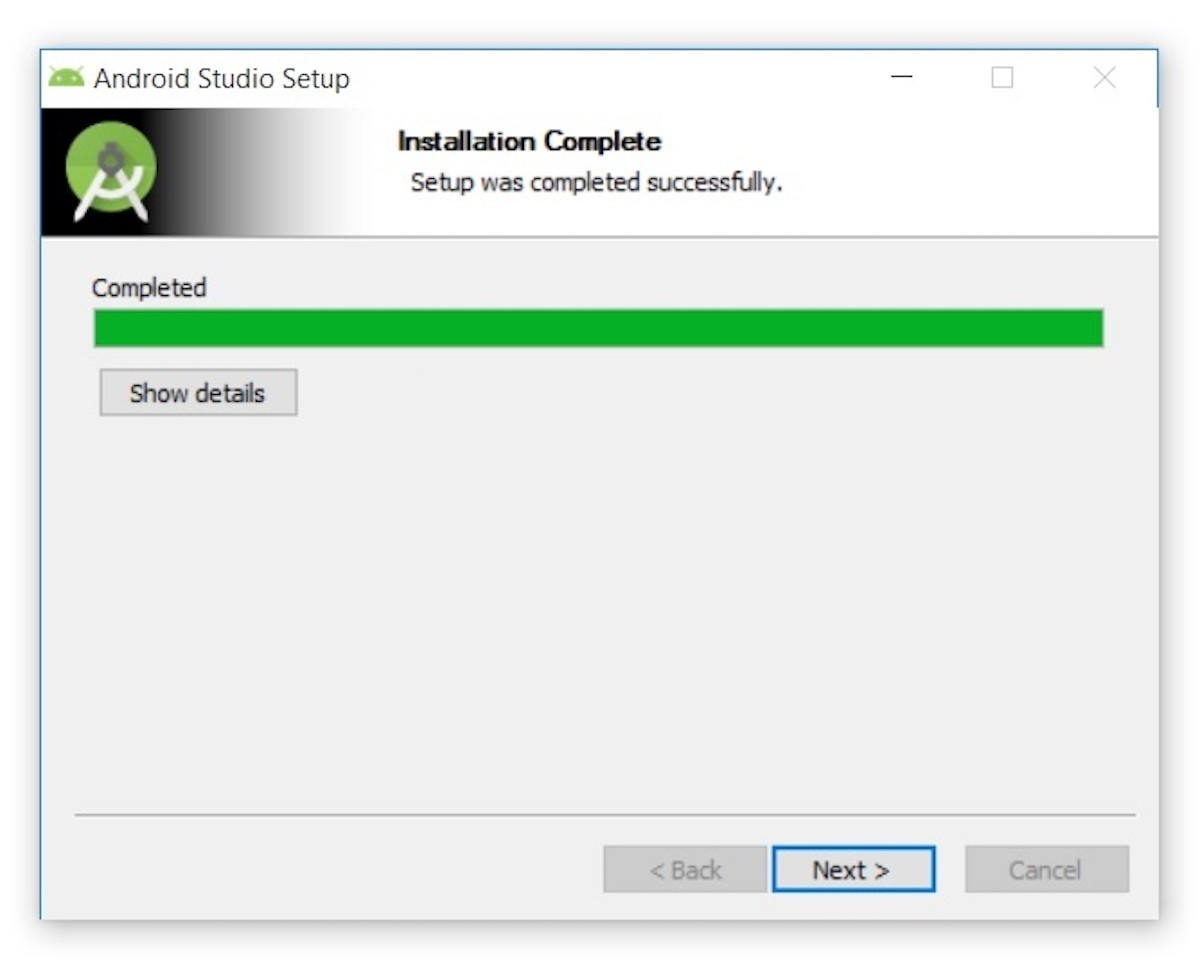
\includegraphics[width=4cm]{figures/installas/6.jpg}
		\centering
		\caption{Proses instalasi selesai.}
	\end{figure}
	\item Kemudian centang Start Android Studio untuk membuka aplikasinya, lalu klik Finish.
	\begin{figure}[H]
		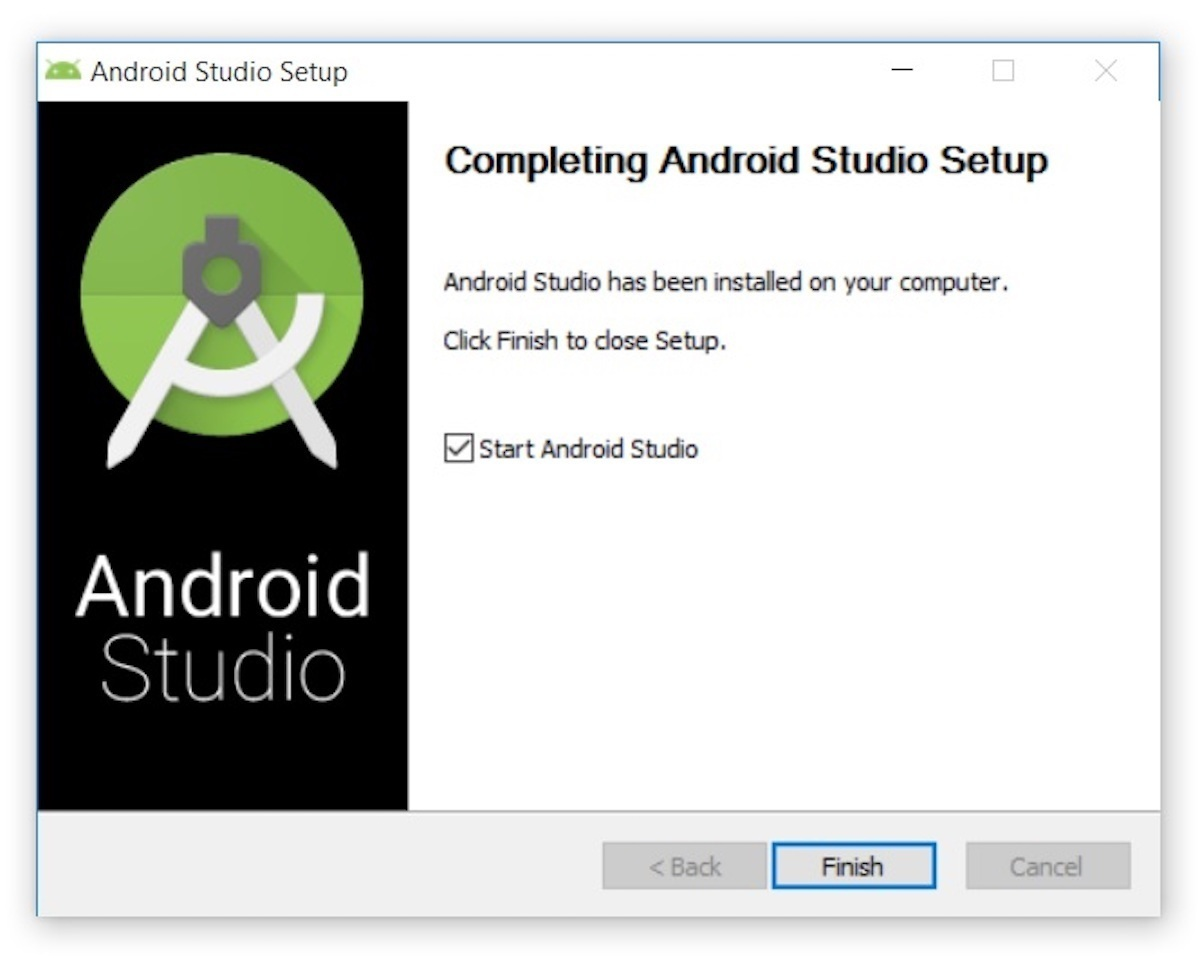
\includegraphics[width=4cm]{figures/installas/7.jpg}
		\centering
		\caption{Jalankan Android Studio.}
	\end{figure}
	\item Ketika Android Studio dijalankan pertama kali, dialog Complete Installation akan muncul dan memberi opsi untuk mengimport setting dari instalasi sebelumnya. Disini kita pilih Do not import settings, lalu klik OK.
	\begin{figure}[H]
		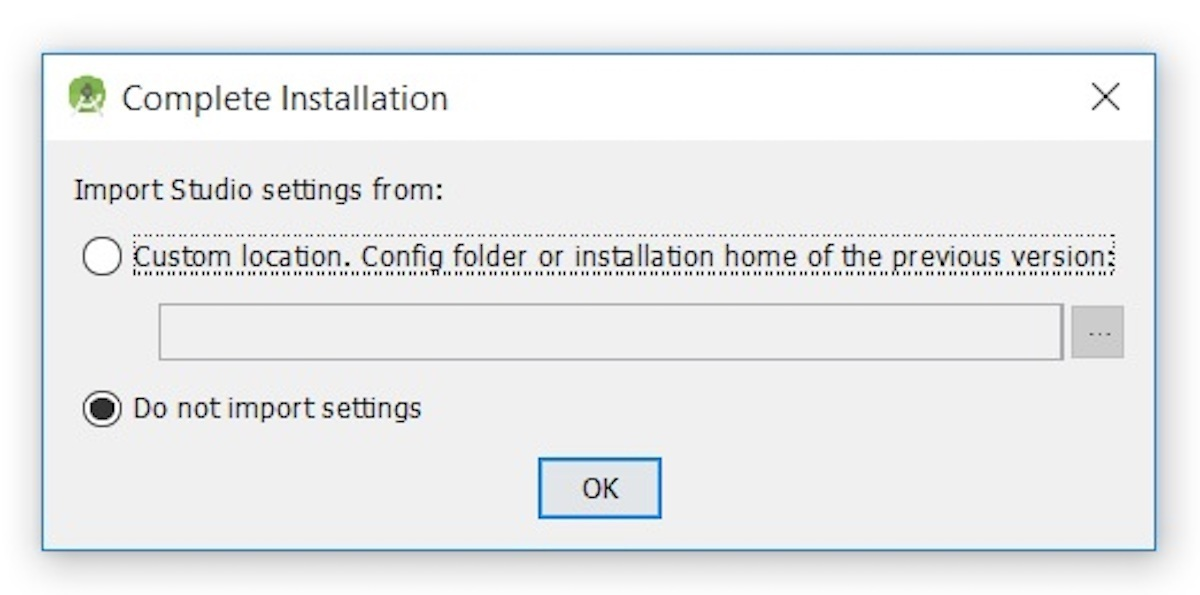
\includegraphics[width=4cm]{figures/installas/8.jpg}
		\centering
		\caption{Import setting instalasi sebelumnya.}
	\end{figure}
	
	\item Kemudian akan muncul splash screen dari Android Studio.
	\begin{figure}[H]
		
\includegraphics[width=4cm]{figures/installas/9.jpg}
		\centering
		\caption{Splash screen Android Studio.}
	\end{figure}
	
	\item Pertama
	\begin{figure}[H]
		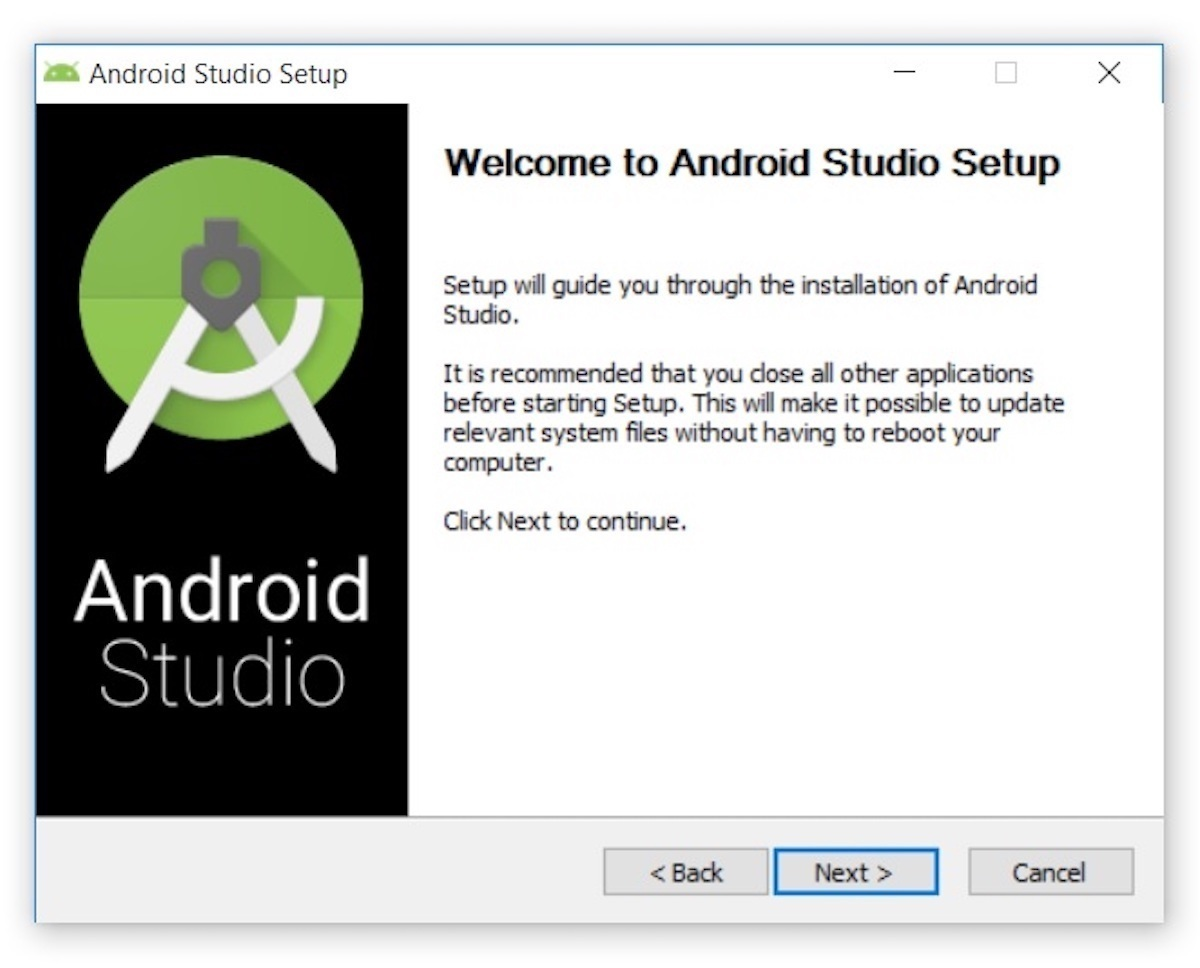
\includegraphics[width=4cm]{figures/installas/1.jpg}
		\centering
		\caption{.}
	\end{figure}
	
	\item Pertama
	\begin{figure}[H]
		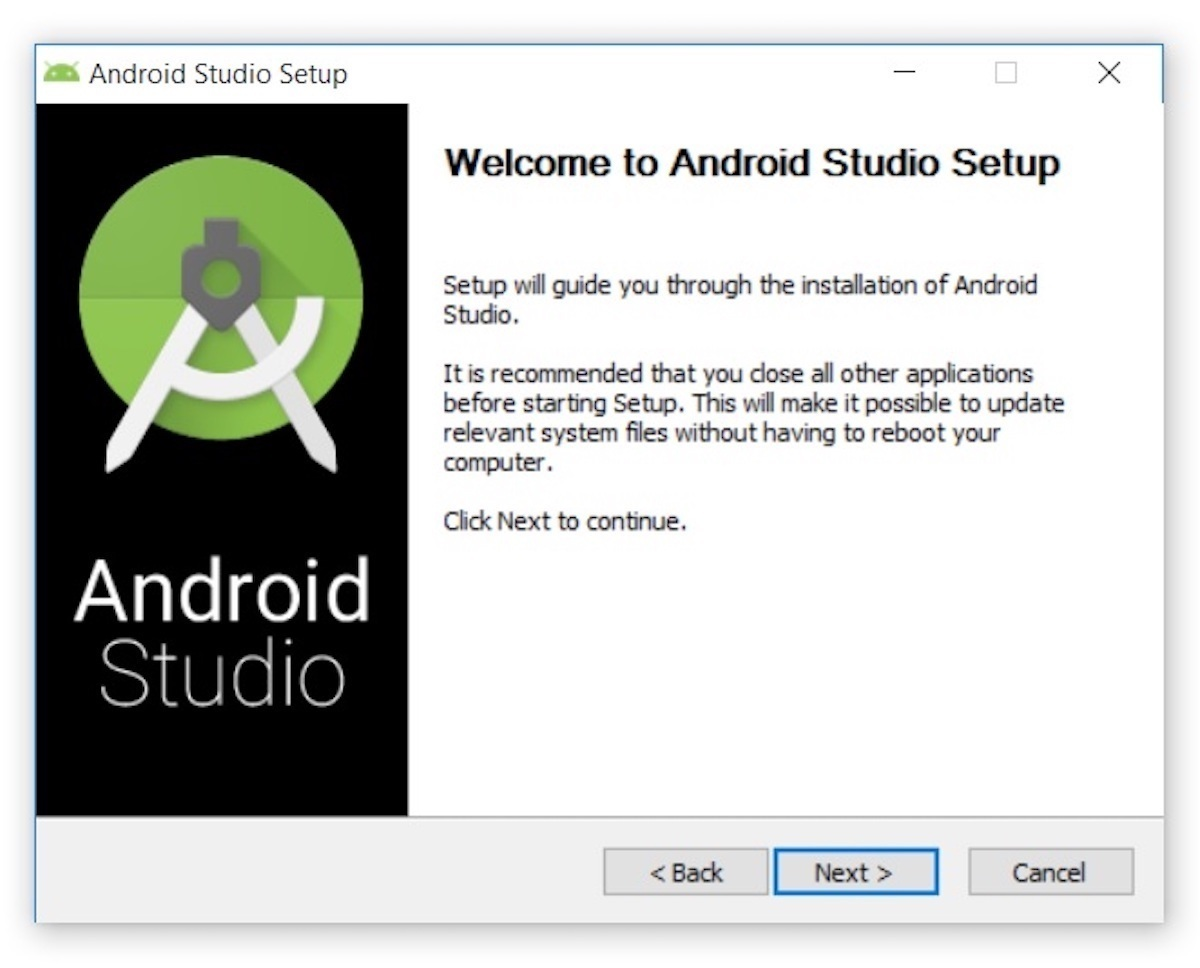
\includegraphics[width=4cm]{figures/installas/1.jpg}
		\centering
		\caption{.}
	\end{figure}
	
	\item Pertama
	\begin{figure}[H]
		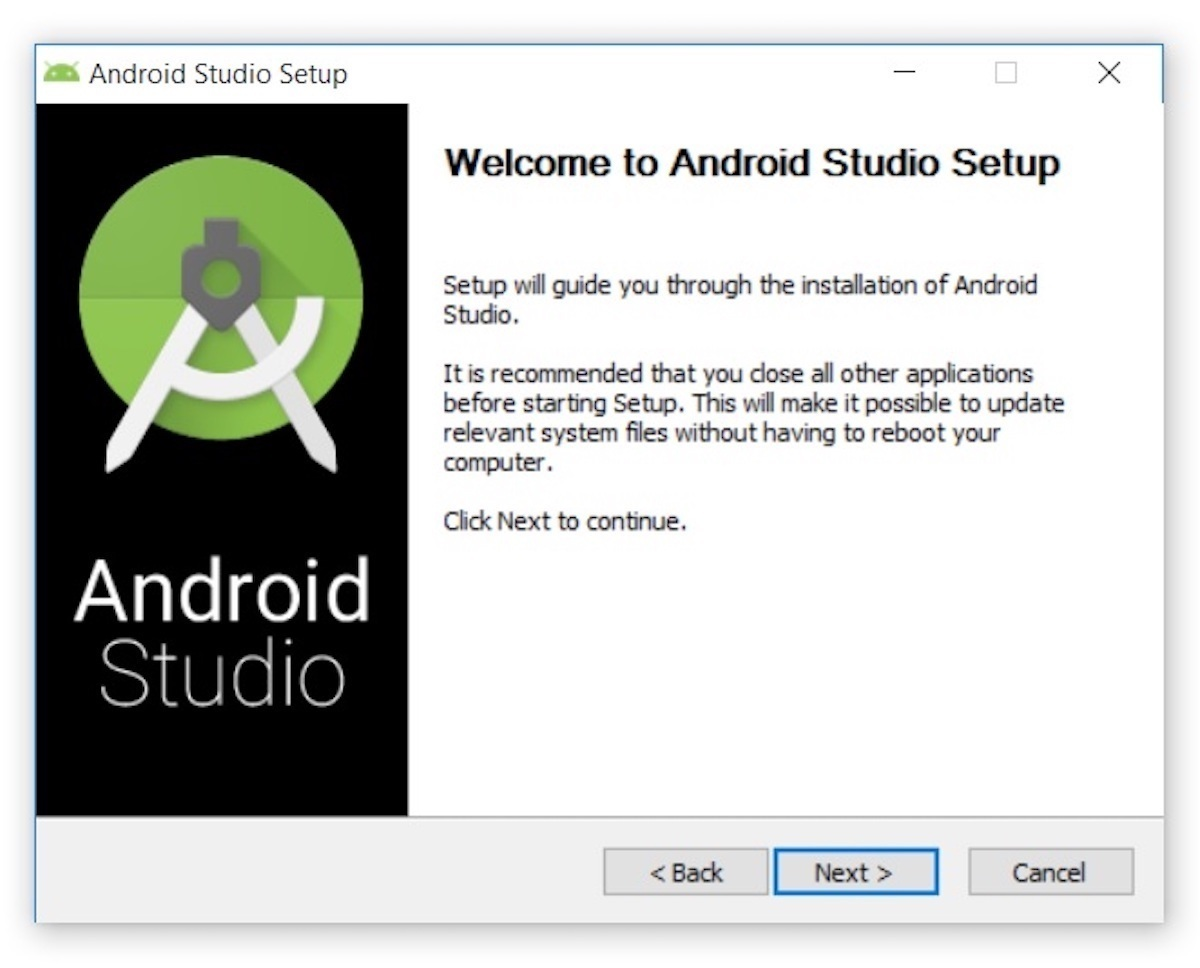
\includegraphics[width=4cm]{figures/installas/1.jpg}
		\centering
		\caption{.}
	\end{figure}
	
	\item Pertama
	\begin{figure}[H]
		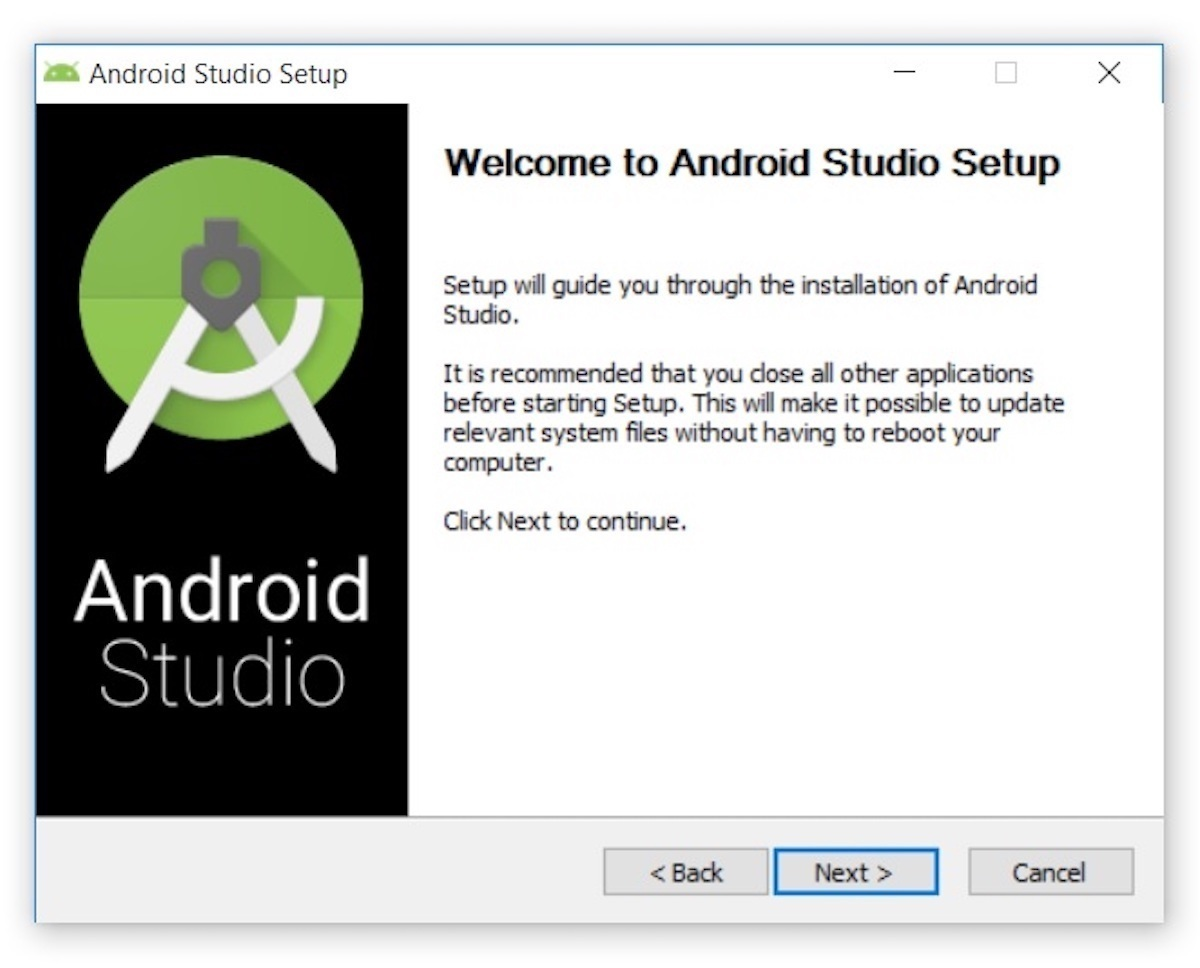
\includegraphics[width=4cm]{figures/installas/1.jpg}
		\centering
		\caption{.}
	\end{figure}
	
	\item Pertama
	\begin{figure}[H]
		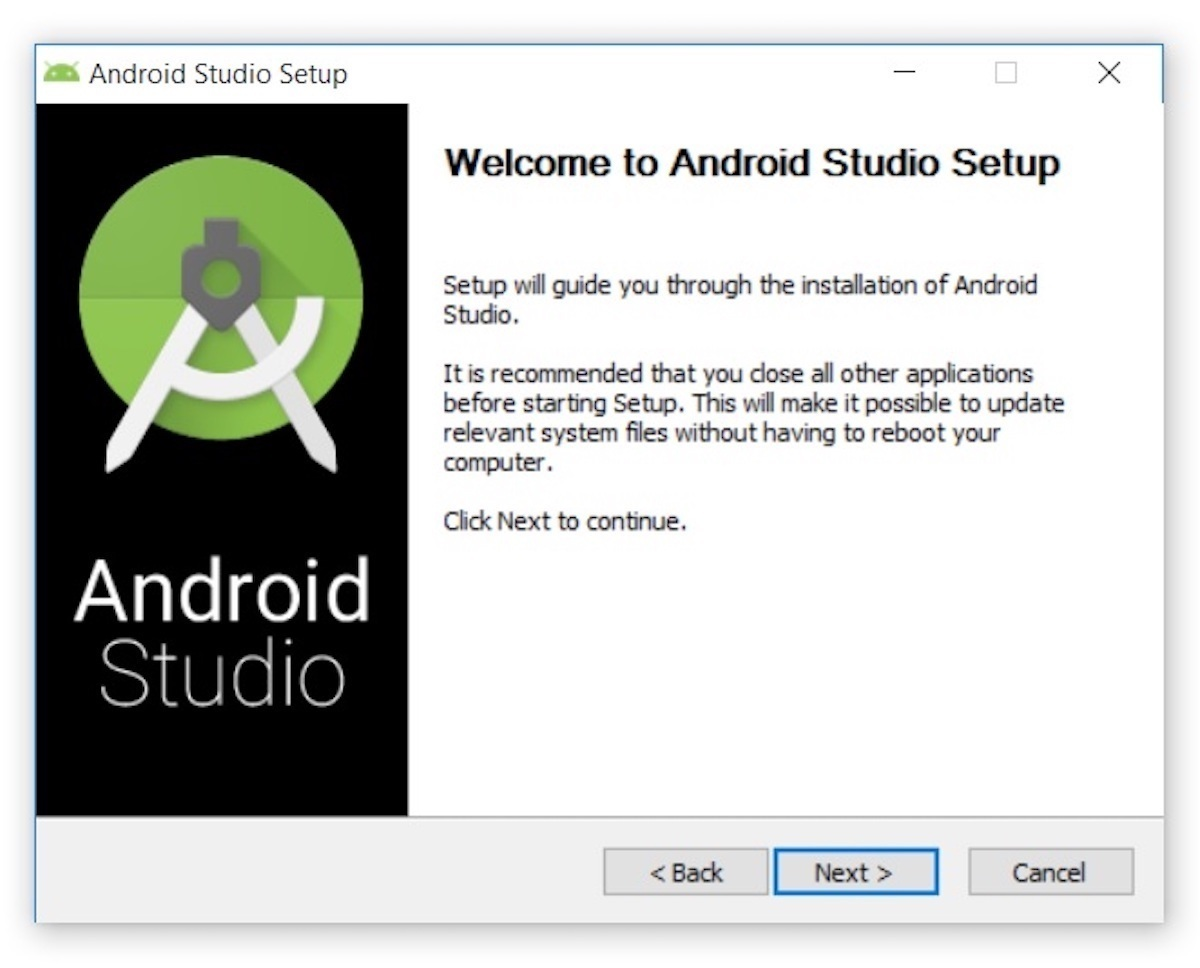
\includegraphics[width=4cm]{figures/installas/1.jpg}
		\centering
		\caption{.}
	\end{figure}
	
	\item Pertama
	\begin{figure}[H]
		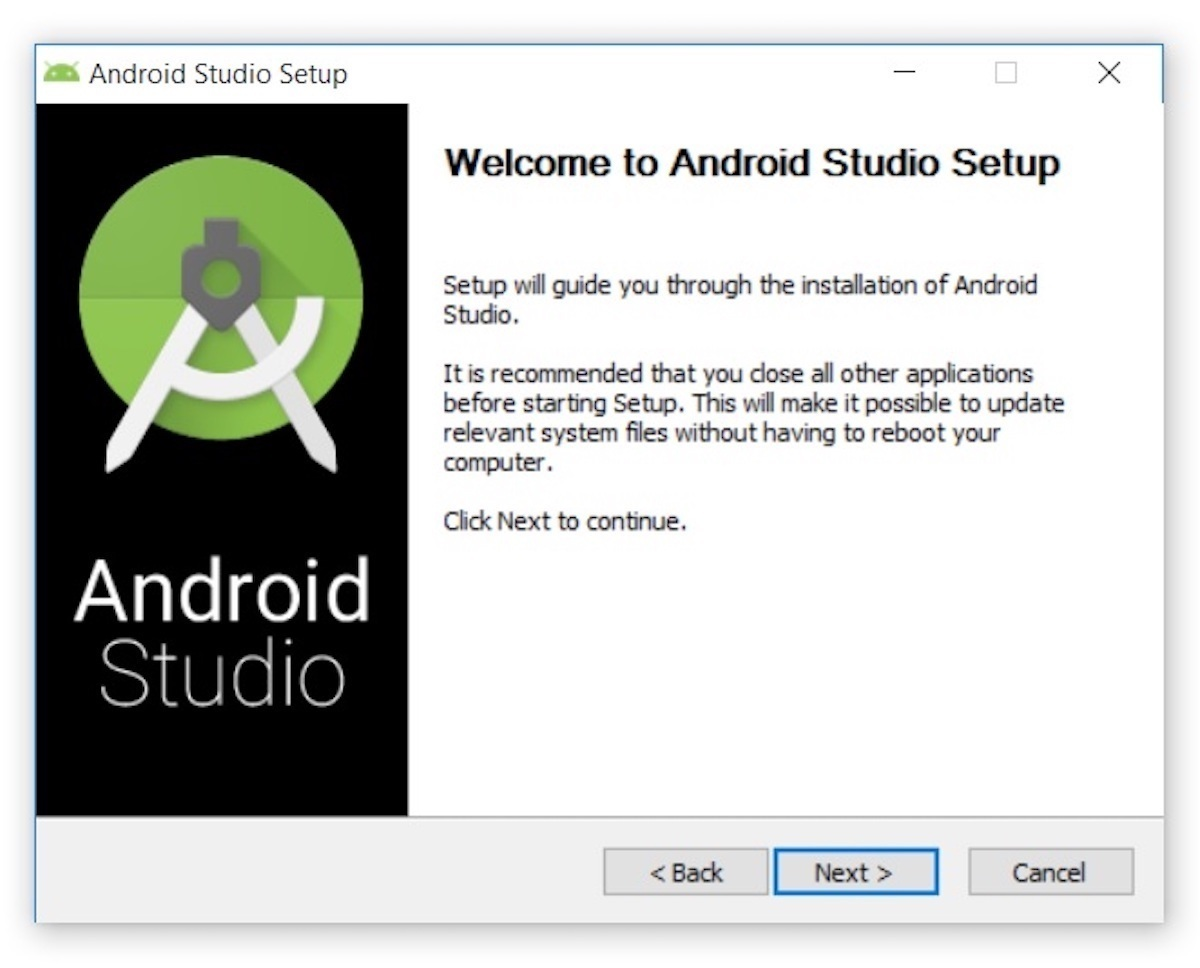
\includegraphics[width=4cm]{figures/installas/1.jpg}
		\centering
		\caption{.}
	\end{figure}
	\begin{figure}[H]
		
\includegraphics[width=4cm]{figures/web/php.png}
		\centering
		\caption{Logo PHP}
	\end{figure}


\subsection{Apa itu PHP?}
PHP adalah bahasa pemrograman yang sering disisipkan ke dalam HTML. PHP memiliki kepanjangan yaitu PHP: Hypertext Preprocessor.Bahasa pemrograman ini menggunakan sistem server-side. Server-side programming adalah jenis bahasa pemrograman yang nantinya script/program tersebut akan dijalankan/diproses oleh server. 

\subsection{Sejarah PHP}
Pada awalnya PHP merupakan kependekan dari Personal Home Page (Situs personal). PHP pertama kali dibuat oleh Rasmus Lerdorf pada tahun 1995. Pada waktu itu PHP masih bernama Form Interpreted (FI), yang wujudnya berupa sekumpulan skrip yang digunakan untuk mengolah data formulir dari web.

Selanjutnya Rasmus merilis kode sumber tersebut untuk umum dan menamakannya PHP/FI. Dengan perilisan kode sumber ini menjadi sumber terbuka, maka banyak pemrogram yang tertarik untuk ikut mengembangkan PHP.

Pada November 1997, dirilis PHP/FI 2.0. Pada rilis ini, interpreter PHP sudah diimplementasikan dalam program C. Dalam rilis ini disertakan juga modul-modul ekstensi yang meningkatkan kemampuan PHP/FI secara signifikan.

Pada tahun 1997, sebuah perusahaan bernama Zend menulis ulang interpreter PHP menjadi lebih bersih, lebih baik, dan lebih cepat. Kemudian pada Juni 1998, perusahaan tersebut merilis interpreter baru untuk PHP dan meresmikan rilis tersebut sebagai PHP 3.0 dan singkatan PHP diubah menjadi akronim berulang PHP: Hypertext Preprocessing.

Pada pertengahan tahun 1999, Zend merilis interpreter PHP baru dan rilis tersebut dikenal dengan PHP 4.0. PHP 4.0 adalah versi PHP yang paling banyak dipakai pada awal abad ke-21. Versi ini banyak dipakai disebabkan kemampuannya untuk membangun aplikasi web kompleks tetapi tetap memiliki kecepatan dan stabilitas yang tinggi.

Pada Juni 2004, Zend merilis PHP 5.0. Dalam versi ini, inti dari interpreter PHP mengalami perubahan besar. Versi ini juga memasukkan model pemrograman berorientasi objek ke dalam PHP untuk menjawab perkembangan bahasa pemrograman ke arah paradigma berorientasi objek. Peladen web bawaan ditambahkan pada versi 5.4 untuk mempermudah pengembang menjalankan kode PHP tanpa menginstal peladen perangkat lunak.

Versi terbaru dan stabil dari bahasa pemograman PHP saat ini adalah versi 7.4.3 yang dirilis pada tanggal 20 Februari 2020

\subsection{Sekilas tentang pembuat PHP : Rasmus Lerdorf}
	\begin{figure}[H]
		
\includegraphics[width=4cm]{figures/web/rasmuslerdorf.jpg}
		\centering
		\caption{Creator PHP Rasmus Lerdorf }
	\end{figure}
Rasmus Lerdorf merupakan seorang programmer yang berasal dari Denmark. Dia membuat dan membantu menginspirasi pengkodean bahasa PHP, terutama pada 2 versi awal yang kemudian dikembangkan secara grup bersama dengan Jim Winstead (Yang membuat blo.gs), Stig Bakken, Shane Caraveo, Andi Gutmans, dan juga Zeev Suraski. sampai sekarang ia terus berkontribusi pada projek.

Lerdorf lahir di pulau disko di daerah Greenland dan kemudian pindah ke Denmark pada awal hidupnya. kelaurganya pindah dari Kanada ke Denmark pada tahun 1980, lalu pindah lagi ke kota King di Ontario pada tahun 1983. Dia lulus dari SMA King City pada tahun 1988, dan pada tahun 1993 lulus dari Universitas Waterloo dengan gelar  Bachelor of Applied Science di bidang teknik desain sistem. Dua juga ikut berkontribusi dalam Apache HTTP Server dan menambahkan clausa Limit pada mSQL DBMS. 

Dari Septermber 2002 sampai November 2009, Lerdorf bekerja di perusahaan Yahoo sebagai Infrastructure Architecture Engineer. Pada tahun 2010 kemudian bergabung ke perusahaan WePay untuk mengembangkan API (Application Programming Interface). dan pada tahun 2011 ia menjadi seorang konsultan untuk beberapa startup. Kemudian pada 22 Februari 2012 ia bergabung dengan Etsy, sebuah website e-commerce yang berfokus pada hal hal vintage. Dan pada tahun 2013, Rasmus bergabung dengan Jelastic sebagai Senior Advisor untuk membantu mereka mengembangkan teknologi baru.

Selain itu Lerdorf juga sering menjadi pembicara dalam konferensi open source di berbagai belahan dunia. Beberapa topik yang sering dia bahas diantaranya adalah security vulnerabilities dan juga tentang PHP.

Pada tahun 2003, ia di beri penghargaan oleh MIT Technology Review sebagai salah satu dari 100 inovator di dunia yang berada dibawah umur 35
\subsection{Website yang menggunakan PHP} 
	\begin{figure}[H]
		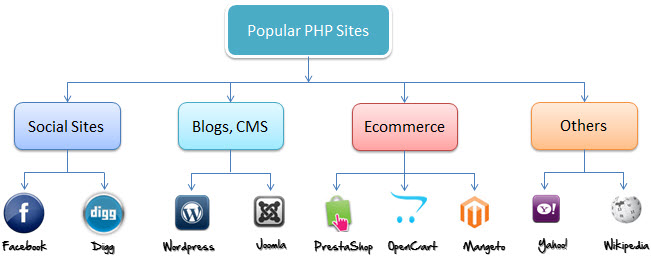
\includegraphics[width=8cm]{figures/web/popularphpsites.jpg}
		\centering
		\caption{Website dengan bahasa PHP}
	\end{figure}

\subsection{Contoh Kode PHP}
	\begin{figure}[H]
		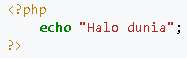
\includegraphics[width=4cm]{figures/web/contohkodingphp.png}
		\centering
		\caption{Program Hello world yang ditulis dengan PHP}
	\end{figure}

\subsection{Kelebihan PHP}
\begin{itemize}
	\item Bahasa pemrograman PHP adalah sebuah bahasa script yang tidak melakukan sebuah kompilasi dalam penggunaannya.
	\item PHP dapat ditemukan di mana - mana
	\item Dalam sisi pengembangan lebih mudah, karena banyaknya developer yang siap membantu dalam pengembangan.
	\item Dalam sisi pemahamanan, PHP adalah bahasa scripting yang paling mudah karena memiliki referensi yang banyak.
	\item PHP adalah bahasa open source yang dapat digunakan di berbagai mesin (Linux, Unix, Macintosh, Windows) dan dapat dijalankan secara runtime melalui console serta juga dapat menjalankan perintah-perintah system
	\item Ringkas
	\item Maintenanace Mudah
\end{itemize}
\subsection{Kekurangan PHP}
\begin{itemize}
	\item Banyak kompetisi, karena PHP adalah bahasa pemrograman yang paling umum
	\item Terkesan kurang prestigious
	\item Tidak ideal jika untuk pengembangan skala besar.
	\item Tidak dapat memisahkan antara tampilan dengan logik dengan baik (Meskipun penggunaan template bisa memperbaikinya)
	\item PHP mempunyai kelemahan security tertentu yang mana jika programmer tidak jeli dalam melakukan pemrograman dan kurang memperhatikan isu dan konfigurasi PHP
\end{itemize}

	\begin{figure}[H]
		
\includegraphics[width=4cm]{figures/web/logocodeigniter.png}
		\centering
		\caption{Logo Codeigniter}
	\end{figure}

\subsection{Pengenalan Codeigniter}

CodeIgniter merupakan aplikasi sumber terbuka yang berupa kerangka kerja PHP dengan model MVC (Model, View, Controller) untuk membangun situs web dinamis dengan menggunakan PHP. CodeIgniter memudahkan pengembang web untuk membuat aplikasi web dengan cepat dan mudah dibandingkan dengan membuatnya dari awal. CodeIgniter dirilis pertama kali pada 28 Februari 2006. Versi stabil terakhir adalah versi 3.1.11
	\begin{figure}[H]
		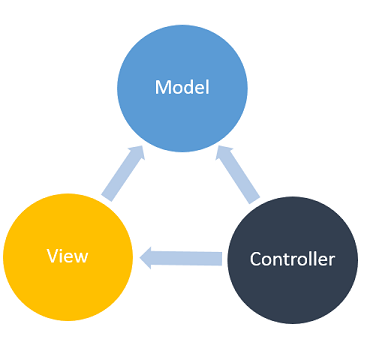
\includegraphics[width=4cm]{figures/web/mvc.png}
		\centering
		\caption{MVC Concept}
	\end{figure}
\subsection{Konsep MVC (Model View dan Controller)}
Model View Controller merupakan suatu konsep yang cukup populer dalam pembangunan aplikasi web, berawal pada bahasa pemrograman Small Talk, MVC memisahkan pengembangan aplikasi berdasarkan komponen utama yang membangun sebuah aplikasi seperti manipulasi data, antarmuka pengguna, dan bagian yang menjadi kontrol aplikasi. Terdapat 3 jenis komponen yang membangun suatu pola MVC dalam suatu aplikasi yaitu: 
\begin{enumerate}
	\item View, merupakan bagian yang menangani logika presentasi. Pada suatu aplikasi web bagian ini biasanya berupa berkas templat HTML, yang diatur oleh controller. View berfungsi untuk menerima dan merepresentasikan data kepada pengguna. Bagian ini tidak memiliki akses langsung terhadap bagian model.
	\item Model, biasanya berhubungan langsung dengan pangkalan data untuk memanipulasi data (insert, update, delete, search), menangani validasi dari bagian controller, tetapi tidak dapat berhubungan langsung dengan bagian view.
	\item Controller, merupakan bagian yang mengatur hubungan antara bagian model dan bagian view, controller berfungsi untuk menerima permintaan dan data dari pengguna kemudian menentukan apa yang akan diproses oleh aplikasi.
\end{enumerate}

\subsection{Kelebihan dan Kekurangan Codeigniter}
\begin{itemize}
	\item Kelebihan
\begin{itemize}
	\item Performa sangat cepat: salah satu alasan tidak menggunakan kerangka kerja adalah karena eksekusinya yang lebih lambat daripada PHP from the scracth, tapi CodeIgniter sangat cepat bahkan mungkin bisa dibilang CodeIgniter merupakan kerangka kerja yang paling cepat dibanding kerangka kerja yang lain
	\item Konfigurasi yang sangat minim
	\item Banyak komunitas: dengan banyaknya komunitas CI ini, memudahkan kita untuk berinteraksi dengan yang lain, baik itu bertanya atau teknologi terbaru
	\item Dokumentasi yang sangat lengkap
\end{itemize}
	\item Kekurangan
\begin{itemize}
	\item CodeIgniter tidak ditujukan untuk pembuatan web dengan skala besar.
	\item Library yang sangat terbatas.
	\item Tidak Adanya Editor Khusus.
\end{itemize}
\end{itemize}
\subsection{Instalasi Codeigniter}


\end{enumerate}


\chapter{Bab 1 : GPS (Global Positioning System)}
\section{GPS (Global Positioning System)}
GPS atau Global Positioning System, merupakan sebuah alat atau sistem yang dapat digunakan untuk menginformasikan penggunanya berada (secara global) di permukaan bumi yang berbasiskan satelit. Data dikirim dari satelit berupa sinyal radio dengan data digital. Dimanapun posisi saat ini, maka GPS bisa membantu menunjukan arah, selama masih terlihat langit. Layanan GPS ini tersedia gratis, bahkan tidak perlu mengeluarkan biaya apapun kecuali membeli GPS recierver-rya.
Awalnya GPS hanya digunakan hanya untuk kepentingan militer, tapi pada tahun 1980-an dapat digunakan untuk kepentingan sipil. GPS dapat digunakan dimanapun juga dalam 24 jam. Posisi unit GPS akan ditentukan berdasarkan titik-titik koordinat derajat lintang dan bujur.

\subsection{Pengertian GPS}
Menurut (Winardi, 2006) adalah sistem untuk menentukan letak di permukaan bumi dengan bantuan penyelarasan (synchronization) sinyal satelit. Sistem ini menggunakan 24 satelit yang mengirimkan sinyal gelombang mikro ke Bumi. Sinyal ini diterima oleh alat penerima di permukaan, dan digunakan untuk menentukan letak, kecepatan, arah, dan waktu. Sistem yang serupa dengan GPS antara lain GLONASS Rusia, Galileo Uni Eropa, IRNSS India. 
Sistem GPS, yang nama aslinya adalah NAVSTAR GPS (Navigation Satellite Timing and Ranging Global Positioning System), mempunyai tiga segmen yaitu : satelit, pengontrol, dan penerima / pengguna. Satelit GPS yang mengorbit bumi, dengan orbit dan kedudukan yang tetap (koordinatnya pasti), seluruhnya berjumlah 24 buah dimana 21 buah aktip bekerja dan 3 buah sisanya adalah cadangan.
Untuk dapat mengetahui posisi seseorang maka diperlukan alat yang diberinama GPS reciever yang berfungsi untuk menerima sinyal yang dikirim dari satelit GPS. Posisi di ubah menjadi titik yang dikenal dengan nama Way-point nantinya akan berupa titik-titik koordinat lintang dan bujur dari posisi seseorang atau suatu lokasi kemudian di layar pada peta elektronik. Sejak tahun 1980, layanan GPS yang dulunya hanya untuk leperluan militer mulai terbuka untuk publik. Uniknya, walau satelit-satelit tersebut berharga ratusan juta dolar, namun setiap orang dapat menggunakannya dengan gratis. (Andy, 2009).
Satelit-satelit ini mengorbit pada ketinggian sekitar 12.000 mil dari permukaan bumi. Posisi ini sangat ideal karena satelit dapat menjangkau area coverage yang lebih luas. Satelit-satelit ini akan selalu berada posisi yang bisa menjangkau semua area di atas permukaan bumi sehingga dapat meminimalkan terjadinya blank spot (area yang tidak terjangkau oleh satelit). Setiap satelit mampu mengelilingi bumi hanya dalam waktu 12 jam. Sangat cepat, sehingga mereka selalu bisa menjangkau dimana pun posisi seseorang di atas permukaan bumi.
GPS reciever sendiri berisi beberapa integrated circuit (IC) sehingga murah dan teknologinya mudah untuk di gunakan oleh semua orang. GPS dapat digunakan utnuk berbagai kepentingan, misalnya mobil, kapal, pesawat terbang, pertanian dan di integrasikan dengan komputer maupun laptop. Berikut beberapa contoh perangkat GPS reciever:
Sejarah GPS
GPS dikembangkan pertama kali sebagai NAVSTAR Global Positioning System (GPS) juga dikenal sebagai NAVigation System with Timing And Ranging GPS. Sistem ini merupakan sistem penentuan posisi berbasis satelit, dan sekaligus merupakan tonggak revolusi bidang pengukuran posisi dan navigasi. 
Sistem GPS pada awalnya merupakan system navigasi ketentaraan yang dirancang, dilaksanakan, dibiayai, dan dikelola oleh Jabatan Pertahanan Amerika Serikat (DoD). Sistem ini dirancang oleh Jabatan Amerika Serikat sejak tahun 1973. Sistem ini adalah hasil gabungan program U.S. Navy TIMATION dan proyek U.S. Air Force 621B di bawah tanggung jawab Joint Program Office (JPO).Satelit GPS yang pertama telah diluncurkan pada tahun 1978. Pada awalnya, penggunaan sistem ini ditujukan bagi pihak tentara Amerika Serikat saja tetapi setelah diluluskan pada Kongres Amerika Serikat, penggunaan sistem penentuan posisi ini terbuka untuk umum. Tujuan utama GPS adalah untuk mewujudkan sistem penentuan posisi di darat, laut, dan udara bagi pihak tentara Amerika Serikat dan sekutunya, namun kemudian sistem ini bebas digunakan oleh semua pengguna. Sistem ini dirancang untuk menggantikan berbagai sistem navigasi yang telah digunakan.

\subsection{Pengenalan GPS}
GPS atau Global Positioning System adalah suatu sistem navigasi satelit yang terdiri dari 24 satelit beroperasi dan 3 satelit cadangan. Ke-24 satelit itu mengorbit bumi pada jarak 20.200 km dan waktu orbit 12 jam, sambil memancarkan sinyal berita gelombang radio. Departemen Pertahanan AS yang mengoperasikan sistem GPS telah mengatur konfigurasi satelit sedemikian rupa, sehingga semua tempat di bumi dapat menerima sinyal dari 4 sampai 10 satelit. Sebagai penunjuk waktu, masing-masing satelit dibekali dengan 4 buah jam atom yang dapat mengukur waktu dengan ketelitian sepermilyar detik. Teknologi GPS sanggup menentukan lokasi manapun di muka bumi dengan ketelitian kurang lebih 1 meter

\subsection{Sistem Satelit GPS}
Untuk menginformasikan posisi user, 24 satelit GPS yang ada di orbit sekitar 12,000 mil di atas kita. Bergerak konstan bergerak mengelilingi bumi 12 jam dengan kecepatan 7,000 mil per jam. Satelit GPS berkekuatan energi sinar matahari, mempunyai baterai cadangan untuk menjaga agar tetap berjalan pada saat gerhana matahari atau pada saat tidak ada energi matahari. Roket penguat kecil pada masing-masing satelit agar dapat mengorbit tepat pada tempatnya.
Satelit GPS adalah milik Departemen Pertahanan (Department of Defense) Amerika, adapun hal-hal lainnya mengenai GPS ini:

\begin{enumerate}
	\item Nama satelit adalah NAVSTAR
	\item GPS satelit pertama kali adalah tahun 1978
	\item Mulai ada 24 satelit dari tahun 1994
	\item Satelit di ganti tiap 10 tahun sekali
	\item GPS satelit beratnya kira-kira 2,000 pounds
	\item Kekuatan transmiter hanya 50 watts atau kurang
\end{enumerate}

Satelit-satelit GPS harus selalu berada pada posisi orbit yang tepat untuk menjaga akurasi data yang dikirim ke GPS reciever, sehingga harus selalu dipelihara agar posisinya tepat. Stasiun-stasiun pengendali di bumi ada di Hawaii, Ascension Islan, Diego Garcia, Kwajalein dan Colorado Spring. Stasiun bumi tersebut selalu memonitor posisi orbit jam jam satelit dan di pastikan selalu tepat.


\subsection{Signal Satelit GPS}
\subsection{Carrier}
Satelite GPS mengirim sinyal dalam dua frekuensi. L1 dengan 1575.42 Mhz dengan membawa dua status pesan dan pseudo-random code untuk keperluan perhitungan wakt. L2 membawa 1227.60 MHz dengan menggunakaan presesi yang lebih akurat karena untuk keperluan militer. 
Daya sinyal radio yang dipancarkan hanya berkisar antara 20-50 Watts. Ini tergolong sangat rendah mengingat jarak antara GPS dan satelit sampai 12.000 mil. Sinyal dipancarkan secara line of sight (LOS), dapat melewati awan, kaca tapi tidak dapat benda padat seperti gedung, gunung

\subsection{Pseudo-Random Codes}
GPS yang digunakan untuk publik akan memantau frekuensi L1 pada UHF (UltraHigh Frequency) 1575,42 MHz. Sinyal L1 yang dikirimkan akan memiliki pola-pola kode digital tertentu yang disebut sebagai pseudorandom. Sinyal yang dikirimkan terdiri dari dua bagian yaitu kode Protected(P) dan Coarse/Acquisition(C/A). Kode yang dikirim juga unik antar satelit, sehingga memungkinkan setiap receiver untuk membedakan sinyal yang dikirim oleh satu satelit dengan satelit lainnya. Beberapa kode Protected (P) juga ada yang diacak, agar tidak dapat diterima oleh GPS biasa. Sinyal yang diacak ini dikenal dengan istilah Anti Spoofing, yang biasanya digunakan oleh GPS khusus untuk keperluan tertentu seperti militer

\subsection{Navigation Message}
Ada sinyal frekuensi berkekuatan lemah yang di tambahkan pada kode L1 yang memberikan informasi tentang orbit satelit, clock corectionnya dan status sistem lainnya.

\subsection{Cara Kerja GPS}
Setiap daerah di atas permukaan bumi ini minimal terjangkau oleh 3-4 satelit.Pada prakteknya, setiap GPS terbaru bisa menerima sampai dengan 12 chanel satelit sekaligus. Kondisi langit yang cerah dan bebas dari halangan membuat GPS dapat dengan mudah menangkap sinyal yang dikirimkan oleh satelit. Semakin banyak satelit yang diterima oleh GPS, maka akurasi yang diberikan juga akan semakin tinggi.
Cara kerja GPS secara logik ada 5 langkah:
\begin{enumerate}
	\item Memakai perhitungan “triangulation” dari satelit.
	\item Untuk perhitungan “triangulation”, GPS mengukur jarak menggunakan travel time sinyal radio.
	\item Untuk mengukur travel time, GPS memerlukan memerlukan akurasi waktu yang tinggi.
	\item Untuk perhitungan jarak, kita harus tahu dengan pasti posisi satelit dan ketingian pada orbitnya.
	\item Terakhir harus menggoreksi delay sinyal waktu perjalanan di atmosfer sampai diterima receiver.
\end{enumerate}

Satelit GPS berputar mengelilingi bumi selama 12 jam di dalam orbit yang akurat dia dan mengirimkan sinyal informasi ke bumi. GPS reciever mengambl informasi itu dan dengan menggunakan perhitungan “triangulation” menghitung lokasi user dengan tepat. GPS reciever membandingkan waktu sinyal di kiirim dengan waktu sinyal tersebut di terima. Dari informasi itu didapat diketahui berapa jarak satelit. Dengan perhitungan jarak jarakGPS reciever dapat melakukan perhitungan dan menentukan posisi user dan menampilkan dalam peta elektronik.

Sebuah GPS reciever harus mengunci sinyal minimal tiga satelit untuk memenghitung posisi 2D (latitude dan longitude) dan track pergerakan. Jika GPS receiver dapat menerima empat atau lebih satelit, maka dapat menghitung posisi 3D (latitude, longitude dan altitude). Jika sudah dapat menentukan posisi user, selanjutnya GPS dapat menghitung informasi lain, seperti kecepatan, arah yang dituju, jalur, tujuan perjalanan, jarak tujuan, matahari terbit dan matahari terbenam dan masih banyak lagi. 
Satelit GPS dalam mengirim informasi waktu sangat presesi karena Satelit tersebut memakai jam atom. Jam atom yang ada pada satelit jalam dengan partikel atom yang di isolasi, sehingga dapat menghasilkan jam yang akurat dibandingkan dengan jam biasa.
Perhitungan waktu yang akurat sangat menentukan akurasi perhitungan untuk menentukan informasi lokasi kita. Selain itu semakin banyak sinyal satelit yang dapat diterima maka akan semakin presesi data yang diterima karena ketiga satelit mengirim pseudo-random code dan waktu yang sama.

Ketinggian itu menimbulkan keuntungan dalam mendukung proses kerja GPS, bagi kita karena semakin tinggi maka semakin bersih atmosfer, sehingga gangguan semakin sedikit dan orbit yang cocok dan perhitungan matematika yang cocok. Satelit harus teptap pada posisi yang tepat sehingga stasiun di bumi harus terus memonitor setiap pergerakan satelit, dengan bantuan radar yang presesi salalu di cek tentang altitude, posision dan kecepatannya.

\subsection{Sistem koordinat pada GPS}
Pengenalan tentang sistem koordinat sangat penting agar dapat menggunakan GPS secara optimum. Setidaknya ada dua klasifikasi tentang sistem koordinat yang dipakai oleh GPS maupun dalam pemetaan yaitu : sistem koordinat global yang biasa disebut sebagai koordinat geografi dan sistem koordinat di dalam bidang proyeksi.
Koordinat geografi diukur dalam lintang dan bujur dalam besaran derajad desimal, derajad menit desimal, atau derajad menit detik Lintangdiukur terhadap equator sebagai titik nol (0\degree  sampai 90\degree  positif kearah utara dan 0\degree  sampai 90\degree  negatif kearah selatan). Bujur diukur berdasarkan titik nol di Greenwich 0\degree  sampai 180\degree  kearah timur dan 0\degree  sampai 180\degree  kearah barat. 
Koordinat di dalam bidang proyeksi merupakan koordinat yang dipakai pada sistem proyeksi tertentu. Umumnya berkait erat dengan sistem proyeksinya, walaupun adakalanya (karena itu memungkinkan) digunakan koordinat geografi dalam bidang proyeksi. Beberapa sistem proyeksi yang lazim digunakan di Indonesia di antaranya adalah : proyeksi Merkator, Transverse Merkator, Universal Tranverse Merkator (UTM), Kerucut Konformal. Masing-masing sistem tersebut ada kelebihan dan kekurangan, dan pemilihan proyeksi umumnya didasarkan pada tujuan peta yang akan dibuat. Dari beberapa sistem proyeksi tersebut, proyeksi Tranverse Merkator dan proyeksi Universal Tranverse Merkator-lah yang banyak dipakai di Indonesia. Peta-peta produksi Dinas Hidro Oseanografi (Dishidros) umumnya menggunakan proyeksi Tranverse Merkator dengan sistem koordinat Geografi atau UTM atau gabungan keduanya. Sedangkan peta-peta produksi Bakosurtanal umumnya menggunakan proyeksi UTM dengan sistem koordinat UTM atau Geografi atau gabungan keduanya.

Sistem koordinat dalam bidang proyeksi tidak dapat terlepas daridatumyang digunakan. Ada dua macamdatum yang umum digunakan dalam perpetaan yaitudatumhorisontal dandatumvertikal. Datum horisontal dipakai untuk menentukan koordinat peta (X,Y), sedangkan datum vertikal untuk menentukan elevasi (peta topografi) ataupun kedalaman (peta batimetri). Perhitungan dilakukan dengan transformasi matematis tertentu. Dengan demikian transformasi antar datum, antar sistem proyeksi, dan antar sistem koordinat dapat dilakukan. Untuk datum horisontal, peta umumnya menggunakan datum Padang (ID-74) untuk peta-peta Bakosurtanal, dan menggunakan datum Jakarta (Batavia) untuk peta-peta Dishidros

\subsection{Cara sinyal dapat menentukan lokasi}
Sinyal yang dikirimkan oleh satelit ke GPS akan digunakan untuk menghitung waktu perjalanan (travel time). Waktu perjalanan ini sering juga disebut sebagai Time of Arrival (TOA). Sesuai dengan prinsip fisika, bahwa untuk mengukur jarak dapat diperoleh dari waktu dikalikan dengan cepat rambat sinyal.

Maka, jarak antara satelit dengan GPS juga dapat diperoleh dari prinsip fisika tersebut. Setiap sinyal yang dikirimkan oleh satelit akan juga berisi informasi yang sangat detail, seperti orbit satelit, waktu, dan hambatan di atmosfir. Satelit menggunakan jam atom yang merupakan satuan waktu paling presisi. 

Untuk dapat menentukan posisi dari sebuah GPS secara dua dimensi (jarak), dibutuhkan minimal tiga buah satelit. Empat buah satelit akan dibutuhkan agar didapatkan lokasi ketinggian (secara tiga dimensi). Setiap satelit akan memancarkan sinyal yang akan diterima oleh GPS receiver. Sinyal ini akan dibutuhkan untuk menghitung jarak dari masingmasing satelit ke GPS. Dari jarak tersebut, akan diperoleh jari-jari lingkaran jangkauan setiap satelit. Lewat perhitungan matematika yang cukup rumit, interseksi (perpotongan) setiap 21lingkaran jangkauan satelit tadi akan dapat digunakan untuk menentukan lokasi dari GPS di permukaan bumi.

\subsection{Penentuan Posisi dengan GPS}
Pada dasarnya penentuan posisi dengan GPS adalah pengukuran jarak secara bersama-sama ke beberapa satelit (yang koordinatnya telah diketahui) sekaligus. Untuk menentukan koordinat suatu titik di bumi,receiver setidaknya membutuhkan 4 satelit yang dapat ditangkap sinyalnya dengan baik. Secaradefault posisi atau koordinat yang diperoleh bereferensi keglobal datum yaitu World Geodetic System 1984 atau disingkat WGS'84.

Secara garis besar penentuan posisi dengan GPS ini dibagi menjadi dua metode yaitumetode absolut dan metode relatif. 
\begin{enumerate}
	\item Metode absolut atau juga dikenal sebagaipoint positioning, menentukan posisi hanya berdasarkan pada 1 pesawat penerima (receiver) saja. Ketelitian posisi dalam beberapa meter (tidak berketelitian tinggi) dan umumnya hanya diperuntukkan bagi keperluan navigasi. 
	\item Metode relatif atau sering disebutdifferentialpositioning, menetukan posisi dengan menggunakan lebih dari sebuah receiver. Satu GPS dipasang pada lokasi tertentu dimuka bumi dan secara terus menerus menerima sinyal dari satelit dalam jangka waktu tertentu dijadikan sebagai referensi bagi yang lainnya. Metode ini menghasilkan posisi berketelitian tinggi (umumnya kurang dari 1 meter) dan diaplikasikan untuk keperluan survei geodesi ataupun pemetaan yang memerlukan ketelitian tinggi.
\end{enumerate}

Untuk keperluan survei di wilayah terumbu karang, metode absolut yang menggunakan single receiver tipe navigasi rasanya sudah cukup memadahi. Akan tetapi bila ingin mempelajari tentang pergeseran terumbu dari waktu ke waktu misalnya, diperlukan metode relatif dengan menggunakan receiver tipe geodetic. Perbincangan selanjutnya akan lebih ke penentuan posisi dengan GPS receivertipe navigasi. 

Beberapa kesalahan dalam penentuan posisi dengan metode absolut ini antara lain disebabkan oleh : efekmultipath,efekselective availability (SA),maupun kesalahan karena ketidaksinkronan antarapeta kerja dansettingyang dilakukan saat menggunakan GPS. 

\begin{enumerate}
	\item Multipath adalah fenomena dimana sinyal dari satelit tiba di anttenna receivermelalui dua atau lebih lintasan yang berbeda. Hal ini biasa terjadi jikalau kita melakukan pengukuran posisi di lokasi-lokasi yang dekatdengan benda reflektif, seperti di samping gedung tinggi, di bawah kawat transmisi tegangan tinggi atau lainnya. Untuk mengatasinya : hindari pengamatan dekat benda reflektif, pakai satelit yang benar-benar baik saja, lakukan pengukuran berulang-ulang dan dirata-rata hasilnya. 
	\item SA adalah teknik pemfilteran yang diaplikasikan untuk memproteksi ketelitian tinggi GPS bagi khalayak umum dengan cara mengacak sinyal - sinyal dari satelit terutama yang berhubungan dengan informasi waktu. Koreksinya hanya dapat dilakukan oleh pihak yang berwenang mengelola GPS ataupun pihak militer Amerika saja. Pihak-pihak lain yang mempunyai ijin untuk menggunakan data berketelitian tinggi biasanya juga diberi tahu cara koreksinya. SA ini merupakan sumber kesalahan paling besar bagi penentuan posisi dengan metode absolut. Namun dengan menerapkan metode relatif (differential positioning) kesalahan tersebut dapat dikurangi. Selain itu belum lama ini pihak militer Amerika telah merevisi kebijakan dalam menerapkanSA ini sehingga saat ini dengan metode absolut-pun ketelitiannya sudah sangat baik dibanding sebelumnya (sudah tidak dalam puluhan meter lagi kesalahannya). Ketidak akuratan posisi karenasettingreceiver yang tidak pas ini hanya dapat diatasi dengan menge-set parameter GPS saat dipakai sesuai dengan parameter peta kerja yang dipergunakan. Hal tersebut biasanya terkait dengan sistem proyeksi dan koordinat, serta datum yang digunakan dalam peta kerja
\end{enumerate}

\subsection{Manfaat GPS}
Dengan menggunakan GPS, seseorang dapat menandai semua lokasi yang pernah di kunjungi. Ada banyak manfaat yang bisa diambil jika seseorang mengetahui waypoint dari suatu tempat. Pertama, orang dapat memperkirakan jarak lokasi yang akan dituju dengan lokasi asal. GPS keluaran terakhir dapat memperkirakan jarak pengguna ke tujuan, sampai estimasi lamanya perjalanan dengan kecepatan aktual yang sedang pengguna tersebut tempuh. Kedua, lokasi di daratan memang cukup mudah untuk dikenali dan diidentifikasi. Namun, jika seseorang kebetulan menemui tempat memancing yang sangat baik di tengah lautan ataupun tempat melihat matahari terbenam yang baik di puncak gunung, bagaimana cara menandai lokasi tersebut agar orang tersebut dapat balik lagi ke lokasi itu di kemudian hari tanpa tersesat. Di saat seperti inilah sebuah GPS akan menunjukkan manfaatnya. 

Dengan teknologi GPS dapat digunakan untuk beberapa keperluan sesuai dengan tujuannya. GPS dapat digunakan oleh peneliti, olahragawan, petani, tentara, pilot, petualang, pendaki, pengantar barang, pelaut, kurir, penebang pohon, pemadam kebakaran dan orang dengan berbagai kepentingan untuk meningkatkan produktivitas, keamanan, dan untuk kemudahan.

Dari beberapa pemakaian di atas dikategorikan menjadi: 
\begin{enumerate}
	\item Lokasi, digunakan untuk menentukan dimana lokasi suatu titik dipermukaan bumi berada. 
	\item Navigasi, membantu mencari lokasi suatu titik di bumi. 
	\item Tracking, membantu untuk memonitoring pergerakan obyek.
	\item Membantu memetakan posisi tertentu, dan perhitungan jaringan terdekat. 
	\item Timing, dapat dijadikan dasar penentuan jam seluruh dunia, karena memakai jam atom yang jauh lebih presesi di banding dengan jam biasa.
\end{enumerate}

\subsection{Model dan Interkoneksi GPS}
Sebuah GPS juga memiliki firmware yang bisa di-upgrade. Upgrade firmware ini biasanya disediakan pada site produsen GPS tersebut. Upgrade firmware biasanya menggunakan kabel yang dibundel atau-pun tersedia sebagai asesoris. Kabel ini juga ternyata bisa digunakan untuk menghubungkan GPS ke komputer (baik itu notebook, PC, maupun PDA dengan sedikit bantuan konverter). Software GPS yang tersedia untuk berbagai platform tersebut juga cukup banyak. Dengan software tersebut, dapat dengan mudah mengunduh informasi dari GPS. Memori sebuah GPS memang relatif terbatas, sehingga kemampuan ekstra untuk menyimpan informasi yang pernah ditempuh ke PC/PDA (yang biasanya memiliki memori lebih besar) tentu akan sangat menyenangkan. Untuk media komunikasi GPS dengan hardware lain selain kabel, model GPS sekarang juga ada yang dilengkapi dengan Bluetooth, Infrared.
Berdasarkan fisik, model GPS dibagi menjadi beberapa tipe antara lain model portable/handheld(ukurannya menyerupai ponsel), ada yang lebih besar (biasanya digunakan di mobil/kapal), ada pula yang meng-gunakan interfacekhusus untuk dikoneksikan ke notebook maupun PDA (Palm, Pocket PC maupun Nokia Com-municator). 

GPS untuk keperluan diluar ruangan biasanya juga dilengkapi dengan perlindungan anti air dan tahan ben-turan. Beberapa GPS keluaran terakhir bahkan sudah menyediakan layar warna dan kemampuan komunikasi radio jarak pendek (FRS/Family Radio Service). Tentu saja, semakin banyak feature yang ditawarkan pada sebuah GPS maka semakin tinggi pula harganya

\subsection{Istilah-istilah yang Penting pada GPS}
Beberapa istilah penting yang penting untuk diketahui yang berhubungan dengan GPS :
\begin{enumerate}
	\item Waypoint : Istilah yang digunakan oleh GPS untuk suatu lokasi yang telah ditandai. Waypoint terdiri dari koordinat lintang (latitude ) dan bujur (longitude ). Sebuah waypoint biasa digambarkan dalam bentuk titik dan simbol sesuai dengan jenis lokasi. 
	\item Mark : Menandai suatu posisi tertentu pada GPS. Jika menandai lokasi menjadi waypoint,maka dikatakan telah melakukan marking. 
	\item Route : Kumpulan waypoint yang ingin seseorang tempuh secara berurutan dan dimasukkan ke dalam GPS.
	\item Track :  Arah perjalanan yang sedang ditempuh dengan menggunakan GPS. Biasanya digambarkan berupa garis pada display GPS.
	\item Elevation : Istilah pada GPS untuk menentukan ketinggian. Ada dua jenis pengukur ketinggian pada GPS, yaitu menggunakan alat klasik ‘barometer ’ atau menggunakan perhitungan satelit. Pengukuran ketinggian menggunakan barometer jauh lebih akurat di udara bebas,namun tidak bisa bekerja dalam pesawat atau ruang vakum lainnya.Ini disebabkan oleh perbedaan tekanan udara dalam ruang vakum dengan tekanan udara di luar. Pengukuran ketinggian menggunakan satelit akan lebih akurat pada tempat seperti itu
	\item Bearing : Arah/posisi yang ingin dituju. Contohnya, A ingin menuju ke suatu lokasi di posisi B yang letaknya di Utara, maka bearing A dikatakan telah diset ke Utara.
	\item Heading : Arah aktual yang sedang dijalankan. Contohnya, saat menuju ke posisi B tadi, A menemui halangan sehingga harus memutar ke selatan terlebih dahulu, maka heading A pada saat itu adalah selatan.
\end{enumerate}

\subsection{Bagian-bagian Daerah Kerja GPS }
GPS terdiri atas tiga segmen yaitu space segment, control segment, user segment, dengan penjelasan sebagai berikut: 
\begin{enumerate}
	\item Space Segment Space segment terdiri atas konstelasi 24 satelit. Masing-masing satelit mengirimkan sebuah sinyal, yang memiliki sejumlah komponen: dua buah gelombang sinus (yang juga dikenal sebagai carrier frequency / frekuensi pembawa), dua kode digital, dan sebuah pesan navigasi. Pesan kode dan navigasi ditambahkan ke dalam pembawa sebagai modulasi dua fasa biner. Pembawa dan kode digunakan terutama untuk menentukan jarak dari receiver pengguna sampai ke satelit GPS. Pesan nagivasi berisi koordinat (lokasi) satelit sebagai fungsi waktu bersama dengan informasi-informasi lain
	\item Control Segment Segmen kontrol dari sistem GPS terdiri atas jaringan lima stasiun pemantau di seluruh pelosok dunia, dengan stasiun kontrol utama (master control station/MCS) berlokasi di dekat Colorado Springs, Colorado, Amerika Serikat. Tugas utama segmen kontrol operasional adalah menjejaki satelit GPS dengan tujuan untuk menentukan dan memprediksikan lokasi satelit, integritas sistem, jam atom satelit, data atmosfer, perkiraan satelit, dan pertimbangan-pertimbangan lain. Informasi ini kemudian digabungkan dan di-upload ke satelit GPS melalui jalur S-band
	\item User Segment User segment mencakup semua pengguna baik militer maupun sipil. Dengan sebuah penerima GPS yang terhubung dengan antena GPS, seorang pengguna dapat menerima sinyal GPS, yang dapat digunakan untuk menentukan posisi pengguna tersebut di manapun di bumi. Saat ini GPS tersedia bagi siapapun di seluruh dunia tanpa biaya apapun
\end{enumerate}

\subsection{Cara Kerja GPS }
Secara teoritis, GPS bekerja dengan cara mengumpulkan data dari satelit, masing-masing satelit akan memberikan informasi jarak antara lokasi satelit tersebut dengan sebuah titik di bumi (GPS receiver). Dari proses pengambilan lokasi-lokasi tersebut akan diperoleh koordinat-koordinat yang disebut waypoint (garis lintang dan bujur pada peta). Dari semua data itu, lokasi titik (GPS receiver) dapat ditentukan dengan cara menerapkan konsep triangulasi. Konsep triangulasi dapat dianalogikan seperti berikut. A ingin datang ke di Gedung G, A tidak tahu di mana letak gedung itu. Ia hanya punya informasibahwa Gedung G terletak 10 km dari Universitas X, 15 km dari Pasar Y dan 20 km dari Terminal Z. Dengan menggambar tiga lingkaran yang berpusat di Universitas X, Pasar Y dan Terminal Z, masing-masing dengan radius 10, 15 dan 20 km. Di titik perpotongan ketiga lingkaran itulah terletak Gedung G. Dalam hal ini, alat penerima akan berada pada titik potong tiga bidang bola; masing-masing dengan radius sebesar jarak alat penerima ke satelit, dengan satelit itu sebagai pusat bola. Dengan demikian, posisi titik itu dapat diketahui dengan titik perpotongan ketiga lingkaran tersebut.

Pada praktiknya, satelit yang digunakan minimum 3 buah dan satelit keempat dibutuhkan untuk perhitungan sinkronisasi clock dari penerima GPS. Akurasi yang diperoleh dengan metode ini terbatas pada 100 meter untuk komponen horizontal, 156 meter untuk vertikal, dan 340 nanodetik untuk komponen waktu, semua pada tingkat probabilitas sebesar 95\%. Tingkat keakuratan yang rendah ini diakibatkan oleh teknik selective availability, yaitu teknik yang digunakan untuk menurunkan akurasi posisi waktu nyata bagi pengguna yang tak berhak. Dengan keputusan pemerintah Amerika Serikat tanggal 1 Mei 2000 untuk penghentian selective availability, akurasi horizontal dapat naik menjadi 22 meter (dengan tingkat probabilitas 95\%). Untuk lebih lagi meningkatkan akurasi GPS, digunakan metode diferensial, yang menggunakan dua alat penerima bersamaan. Dalam kasus ini, tingkat keakuratan yang diperoleh mencapai beberapa meter saja

\subsection{Menentukan Posisi dari Receiver ke Satelit GPS  }
Sebuah GPS receiver mengetahui lokasi dari satelit dengan cara menghitung seberapa jauh jarak antara satelit dan receiver dengan menggunakan rumus sebagai berikut :
Kecepatan x Waktu = Jarak (2-1)
Keterangan: 
Kecepatan = kecepatan gelombang mikro yang dikirimkan dari satelit, 
Waktu = waktu yang dibutuhkan dari satelit mengirimkan sinyal hingga diterima GPS receiver, 
Jarak = jarak antara satelit dengan GPS receiver. 
Dari diketahui jarak antara receiver dengan satelit, maka dapat ditentukan posisi receiver dengan cara mengirimkan balik sinyal ke satelit sehingga membentuk suatu lingkaran dari ketiga satelit yang ada.
TTFF (Time to First Fix) 
TTFF (Time to First Fix) adalah waktu yang diperlukan oleh sebuah GPS receiver untuk mengetahui posisinya saat ini. TTFF bergantung pada mode boot up mode GPS apakah hot start, warm start, atau cold start.Secara umum factor-faktor yang mempengaruhi boot mode antara lain sebagai berikut
\begin{itemize}
	\item Adanya data almanac dan ephemeris yang valid.
	\item  Kuat sinyal yang diterima receiver. 
	\item Posisi receiver dari tempat terakhir dimana dia fix atau memperoleh data yang valid (sekitar 100 km dari tempat terakhir dia memperoleh data yang valid).
	\item Waktu terakhir fix atau memperoleh data yang valid.
\end{itemize}

Setiap satelit GPS melakukan broadcast pesan navigasi dengan kecepatan 50 bit/s yang berisi kondisi informasi satelit GPS (ditransmisikan pada bagian pertama dari pesan), data ephemeris (ditransmisikan pada bagian kedua dari pesan), dan data almanac (ditransmisikan pada bagian akhir dari pesan). Pesan dikirim dalam frame dimana masing-masing frame memerlukan waktu 30 detik untuk mengirimkan 1500 bit. Setiap frame terdiri 5 subframe dengan lama 6 detik dan panjang 300 bit. Setiap subframe terdiri dari 10 words yang masing-masing terdiri dari 30 bit dengan masing-masing memerlukan 0,6 detik untuk dikirimkan.

Word 1 dan 2 dari setiap subframe memiliki tipe data yang sama. Wordpertama mengindikasikan awal dari sebuah subframe dan digunakan oleh receiver untuk melakukan sinkronisasi dengan pesan navigasi. Word kedua merupakan handover word yang memiliki informasi waktu yang memungkinkan receiver untuk mengidentifikasi subframe dan memberitahukan waktu pengiriman subframe selanjutnya.

Word 3 sampai 10 dari subframe 1 terdiri atas data yang menjelaskan clocksatelit dan hubungan dengan waktu GPS. Word 3 sampai 10 dari subframe 2 dan 3 terdiri dari data ephemeris yang menunjukkan letak pasti dari satelit tersebut. Data ephemeris diperbaharui setiap sekitar 2 jam

Almanac terdiri dari posisi kasar (tidak begitu akurat) dan informasi status dari setiap satelit. Word 3 sampai 10 pada subframe 4 dan 5 terdiri dari sebuah bagian baru dari data almanac. Setiap frame memiliki 1/25 data almanacsehingga diperlukan waktu selama 12,5 menit untuk memperoleh almanackeseluruhan dari tiap satu satelit. Data almanac memiliki beberapa fungsi yakni untuk membantu penemuan satelit pada penyalaan atau membantu untuk memprediksi satelit mana yang terlihat dengan mengizinkan receiver untuk memberikan daftar satelit yang terlihat berdasarkan posisi dan waktu yang tersimpan sehingga mempersingkat waktu akuisisi. Data almanac akan disimpan di non-volatile memory. Sementara itu data ephemeris dari setiap satelit diperlukan untuk menghitung posisi menggunakan satelit tersebut. Jika receiver tidak memiliki data almanac maka akan menyebabkan waktu delay yang lama sebelum memperoleh posisinya yang valid karena dilakukan pencarian terhadap masing-masing satelit merupakan proses yang lambat. Ketika sebuah GPS receiver sudah pernah fix dan dimatikan, posisi dan data yang valid akan disimpan. Ketika receiver dihidupkan kembali, dia akan berusaha untuk menggunakan informasi yang telah tersimpan dalam almanacuntuk memprediksi satelit mana yang terlihat. Jika receiver telah berpindah terlalu jauh atau internalclock sudah tidak aktif (GPS tidak aktif dari 3 hari sebelumnya), maka data yang tersimpan tidak dapat digunakan untuk membantu memprediksi lokasi satelit.

GPS memiliki beberapa mode start up, yaitu: 
\begin{itemize}
	\item Mode Cold Start  : GPS melakukan startup dalam mode ini ketika: 
	\begin{itemize}
		\item Receiver telah berpindah lebih dari 100 km dari lokasi fix terakhir. 
		\item Waktu saat ini tidak akurat atau tidak diketahui. 
		\item Sinyal yang diterima lemah. Satelit yang diprediksi secara fisik ada di atas atau terlihat tetapi receiver tidak bisa melihatnya misalnya karena adanya bangunan yang tinggi atau halangan lainnya
	\end{itemize}
Situasi-situasi seperti di atas memiliki arti bahwa receiver tidak bisa memprediksi dan/atau membuktikan satelit mana yang terlihat. Receiver kemudian mencari semua satelit dan mencoba untuk memperolehnya secara bergantian. TTFF untuk cold start bisa mencapai belasan menit.
	\item Mode Warm Start : GPS melakukan startup dalam mode ini ketika: 
	\begin{itemize}
		\item Tidak ada data ephemeris yang tersimpan.
		\item Waktu saat ini diketahui (GPS pernah aktif dalam tiga hari terakhir). . 
		\item Lokasi saat ini tidak lebih dari 100 km dari lokasi fix terakhir.
		\item Memiliki alamat yang valid. 
		\item Terdapat 4 atau lebih satelit dengan HDOP < 6 dan kekuatan sinyal yang bagus (misalnya satelit memiliki geometri yang bagus dan bisa melihat langit secara langsung). 
	\end{itemize}
Receiver bisa memprediksi satelit mana yang terlihat tetapi perlu untuk memperoleh data ephemeris saat ini terlebih dahulu. TTFF untuk mode start ini biasanya sekitar 45 detik.
	\item Mode Hot Start : GPS receiverstart up dengan mode hot start jika kondisi warm startterpenuhi dan ketika
	\begin{itemize}
		\item Sudah fix dalam 2 jam terakhir.
		\item Receiver memiliki data ephemeris yang valid minimal untuk 5 satelit 
	\end{itemize}
Dalam mode ini, receiver dengan cepat mengetahui satelit yang terlihat dan hanya perlu memperoleh data yang sedikit untuk mengetahui posisinya. TTFF untuk hot start biasanya 22 detik

TTFF bisa juga dipengaruhi oleh konstelasi atau posisi satelit. Semakin banyak satelit dalam lokasi yang bagus mengurangi TTFF dan meningkatkan akurasi. Minimal dibutuhkan 4 satelit untuk fix. Dengan 5 atau lebih dibutuhkan untuk kualitas fix yang lebih bagus. 
GPS bekerja dengan konsep triangulasi. Satelit yang berada tepat di atas (sudut elevasi 90o) memberikan hasil yang lebih tidak akurat dibandingkan dengan satelit dengan sudut elevasi yang lebih rendah. Namun sinyal dari satelit yang terlalu lemah pada langit yang harus melewati atmosfer bumi akan mengurangi akurasi juga.
\end{itemize}

\subsection{Ketidakakuratanpada GPS   }
Sistem GPS telah didesain untuk seakurat mungkin, tetapi masih ada penyimpangan yang terjadi. Ada banyak penyebab dari penyimpangan ini, yaitu :
\begin{enumerate}
	\item Kondisi Atmosfer Kondisi atmosfer yang berubah mengakibatkan kecepatan sinyal GPS berubah karena sinyal tersebut melewati atmosfer bumi dan ionosfer sehingga kecepatan gelombang mikro dari satelit akan berubah, yang akan mempengaruhi perhitungan jarak menjadi tidak akurat.
	\item Ephemeris Error dan Clock Error Sinyal pada GPS membawa informasi tentang error pada ephemeris (posisi secara orbital).
	\item Selective Availabilty Selective Availability (SA) adalah teknik yang digunakan untuk menurunkan akurasi posisi waktu nyata bagi pengguna yang tak berhak, dimana merupakan suatu penyimpangan posisi yang disengaja dari sekitar 0 sampai ribuan kaki ke dalam sinyal navigasi yang ada secara umum. SA ini bisa dihilangkan dengan cara koreksi secara diferrensial.
	\item Multipath Signal yang mengalami pantulan akibat memasuki atmosfer bumi ketika menuju ke antena GPS
	\item Dilution Of Precision (DOP) DOP merupakan sebuah indikator kualitas dari geometri pada konstelasi satelit. Perhitungan sebuah posisi bisa berbeda-beda tergantung pada satelit mana yang sedang digunakan. Perbedaaan geometri satelit bisa memperbesar atau bahkan memperkecil error pada GPS. Semakin besar sudut antara satelit yang satu dengan yang lainnya maka akan memperkecil nilai DOP, dan menghasilkan pengukuran yang lebih baik. Nilai yang tinggi pada DOP berarti mengindikasikan geometri yang buruk pada satelit.
Format Kalimat GPS Perusahaan-perusahaan pembuat GPS memiliki format kalimat masing-masing untuk menyimpan hasil pengukuran GPS, sehingga sulit untuk menggabungkan data dari alat GPS yang berbeda. Masalah yang mirip terjadi saat ingin melakukan antar-muka terhadap berbagai alat yang berbeda, termasuk sistem GPS. Untuk mengatasi masalah ini, banyak peneliti yang membuat format standar untuk berbagai keperluan penggunanya. Format standar yang banyak digunakan saat ini ada empat, yaitu
	\begin{enumerate}
		\item RINEX : RINEX dibuat oleh sekelompok peneliti untuk mengatasi kesulitan mengkombinasikan data biner dari penerima GPS yang berbeda. Data RINEX merupakan format standar ASCII, sehingga memakan tempat yang lebih banyak dalam penyimpanannya
		\item NGS-SP3 : NGS-SP3 dibangun oleh U.S. NGS yang merupakan akronim dari Standard Product 3, yang datanya berupa dokumen ASCII yang berisi data orbital yang presisi dan koreksi clock satelit yang bersangkutan
		\item RTCM SC-104 untuk Layanan DGPS : Format ini merupakan format standar industri untuk mengirimkan koreksi waktu nyata DGPS yang diajukan oleh Radio Technical Commission for Maritime Services untuk memastikan operasi yang efisien dan koreksi pseudorange
		\item NMEA 0183 : NMEA merupakan akronim dari National Marine Electronics Association, yang formatnya diadopsi sebagai format untuk antar-muka alat-alat elektronik kelautan. Format ini juga menggunakan data dalam format ASCII
	\end{enumerate}
GPS yang merupakan kependekan dari Global Positioning SystemGlobal Positioning System, adalah suatu system, adalah suatu systemradio navigasi dan penentuan posisi radio navigasi dan penentuan posisi yang berbasiskan satelit yang dapat digunakan oleh yang berbasiskan satelit yang dapat digunakan oleh banyak banyak orang sekaligus dalam segala cuaca, serta didesain untuk memberikan posisi dan kecepatan tigaorang sekaligus dalam segala cuaca, serta didesain untuk memberikan posisi dan kecepatan tigadimensi yang teliti, dan juga informasi mengenai waktu, secara kontinyu di seluruh duniadimensi yang teliti, dan juga informasi mengenai waktu, secara kontinyu di seluruh dunia(Abidin, 1995).(Abidin, 1995).Selain ituSelain itu Global Positioning SystemGlobal Positioning System(GPS) adalah system untuk menentukan posisi di(GPS) adalah system untuk menentukan posisi dipermukaan bumi dengan bantuan sinkronisasi sinyal satelit. Sistem ini menggunakan satelit permukaan bumi dengan bantuan sinkronisasi sinyal satelit. Sistem ini menggunakan satelit yang mengirimkan sinyal gelombang mikro ke Bumi. Sinyal ini diterima oleh alat penerima diyang mengirimkan sinyal gelombang mikro ke Bumi. Sinyal ini diterima oleh alat penerima dipermukaan, dan digunakan untuk menentukan posisi, kecepatan, arah, dan permukaan, dan digunakan untuk menentukan posisi, kecepatan, arah, dan waktu.waktu.Untuk dapat mengetahui posisi seseorang maka diperlukan alat yang diberinama GPSUntuk dapat mengetahui posisi seseorang maka diperlukan alat yang diberinama GPSreciever yang berfungsi untuk menerima sinyal yang dikirim dari satelit GPS. Posisi di ubahreciever yang berfungsi untuk menerima sinyal yang dikirim dari satelit GPS. Posisi di ubahmenjadi titik yang dikenal dengan nama Way-point nantinya akan berupa titik-titik koordinat menjadi titik yang dikenal dengan nama Way-point nantinya akan berupa titik-titik koordinat lintang dan bujur dari posisi seseorang atau suatu lokasi kemudian di layar pada petalintang dan bujur dari posisi seseorang atau suatu lokasi kemudian di layar pada peta elektronik.
\end{enumerate}

\subsection{SEGMEN PADA PADA SATELIT SATELIT GPS}
Sistem GPS yang nama aslinya NAVSTAR GPS (Sistem GPS yang nama aslinya NAVSTAR GPS (Navigational Satellite Timing and Ranging Navigational Satellite Timing and Ranging Global Positioning SystemGlobal Positioning System) mempunyai tiga segmen yaitu : satelit, pengontrol dan) mempunyai tiga segmen yaitu : satelit, pengontrol danpenerima/pengguna. Satelit GPS yang mengorbit bumi, dengan orbit dan kedudukan yang tetappenerima/pengguna. Satelit GPS yang mengorbit bumi, dengan orbit dan kedudukan yang tetap(koordinatnya pasti).(koordinatnya pasti).
\begin{itemize}
	\item Satelit Satelit Satelit bertugas untuk menerima dan menyimpan data yang ditransmisikan olehSatelit bertugas untuk menerima dan menyimpan data yang ditransmisikan olehstatiun-statiun pengontrol, menyimpan dan menjaga informasi waktu berketelitian tinggi yangstatiun-statiun pengontrol, menyimpan dan menjaga informasi waktu berketelitian tinggi yangditentukan dengan jam atomic di ditentukan dengan jam atomic di satelit dan memancarkan sinyal dan informasi secara kontinyusatelit dan memancarkan sinyal dan informasi secara kontinyuke pesawat (receiver) dari pengguna.ke pesawat (receiver) dari pengguna
	\item PengontrolPengontrolPengontrol bertugas untuk mengendalikan dan mengontorol satelit dari bumi baik Pengontrol bertugas untuk mengendalikan dan mengontorol satelit dari bumi baik untuk mengecek kesahatan satelit, penentuan dan prediksi orbit dan waktu, sinkronisasi waktuuntuk mengecek kesahatan satelit, penentuan dan prediksi orbit dan waktu, sinkronisasi waktuantar satelit, dan mengirim data ke satelit.antar satelit, dan mengirim data ke satelit
	\item PenerimaPenerimaPenerima bertugas menerima data dari satelit dan memprosesnya untuk menentukanPenerima bertugas menerima data dari satelit dan memprosesnya untuk menentukanposisi (posisi dari tiga dimensi yaitu koordinat di bumi plus ketinggian), arah, jarak dan waktuposisi (posisi dari tiga dimensi yaitu koordinat di bumi plus ketinggian), arah, jarak dan waktuyang diperlukan oleh pengguna yang diperlukan oleh pengguna
\end{itemize}

\subsection{Kelebihan GPS}
\begin{enumerate}
	\item Dapat menandai semua lokasi yang pernah dikunjungi oleh pengguna
	\item Dapat memperkirakan jarak lokasi yang dituju oleh pengguna dengan mengetahui lokasiasalnya, GPS juga dapat memperkirakan estimasi lamanya perjalanan dengan kecepatanaktual yang sedang ditempuh oleh pengguna
	\item Dimanapu posisi pengguna, entah itu di tengah laut atau pegunungan, di atas gunungsampai di pusat kota, selama GPS dapat menerima sinyal dari satelit secara langsungtanpa halangan, maka GPS akan selalu memberikan informasi koordinat posisipengguna
\end{enumerate}

\subsection{Kekurangan GPS}
\begin{enumerate}
	\item GPS harus berada di luar ruangan yang menghadap langit terbuka, halangan–halanganseperti pohon, gedung, kaca atau disaat pengguna berada di dalam kendaraan akanmengurangi akurasi sinyal yang diterima oleh receiver GPS, bahkan receiver GPS jugabisa tidakbisa menerima sinyal sama sekali
	\item Banyak gangguan yang dapat menurunkan kualitas sinyal GPS sehingga akanmempengaruhi ketelitian pengukuran, diantaranya adalah delay ionosfer, sinyalmultipath, kesalahan orbital, geometri
	\item Adanya penurunan kualitas sinyal satelit, yaitu penurunan kualitas sinyal yangdikenakan oleh pejabat Amerika Serikat untuk mencegah musuh militer daripenggunaan sinyal GPS yang akurat
	\item Adanya kesalahan orbital, yaitu kesalahan efemeris yang merupakan ketidakakurasianlokasi yang dilaporkan oleh satelit penerima GPS
	\item Kesalahan jam penerima dapat menyebabkan kesalahan waktu
	\item Delay ionosfer, yaitu atmosfer yang mengalami perubahan dalam hal temperatur,tekanan, kelembaban, dan perubahan cuaca, yang menyebabkan sinyal satelit GPSterlambat sampai ke atmosfer
	\item
\end{enumerate}

\chapter{Bab 2 : API,Java dan PHP}
\section{Persiapan dan pengenalan}
\subsection{Instalasi Java}
\subsection{Instalasi Android Studio}
\begin{enumerate}
	\item Kemudian klik dua kali pada installer yang telah di-download untuk memulai proses instalasi. Installer akan menampilkan Android Studio Setup seperti gambar berikut, lalu klik Next. 
	\begin{figure}[H]
		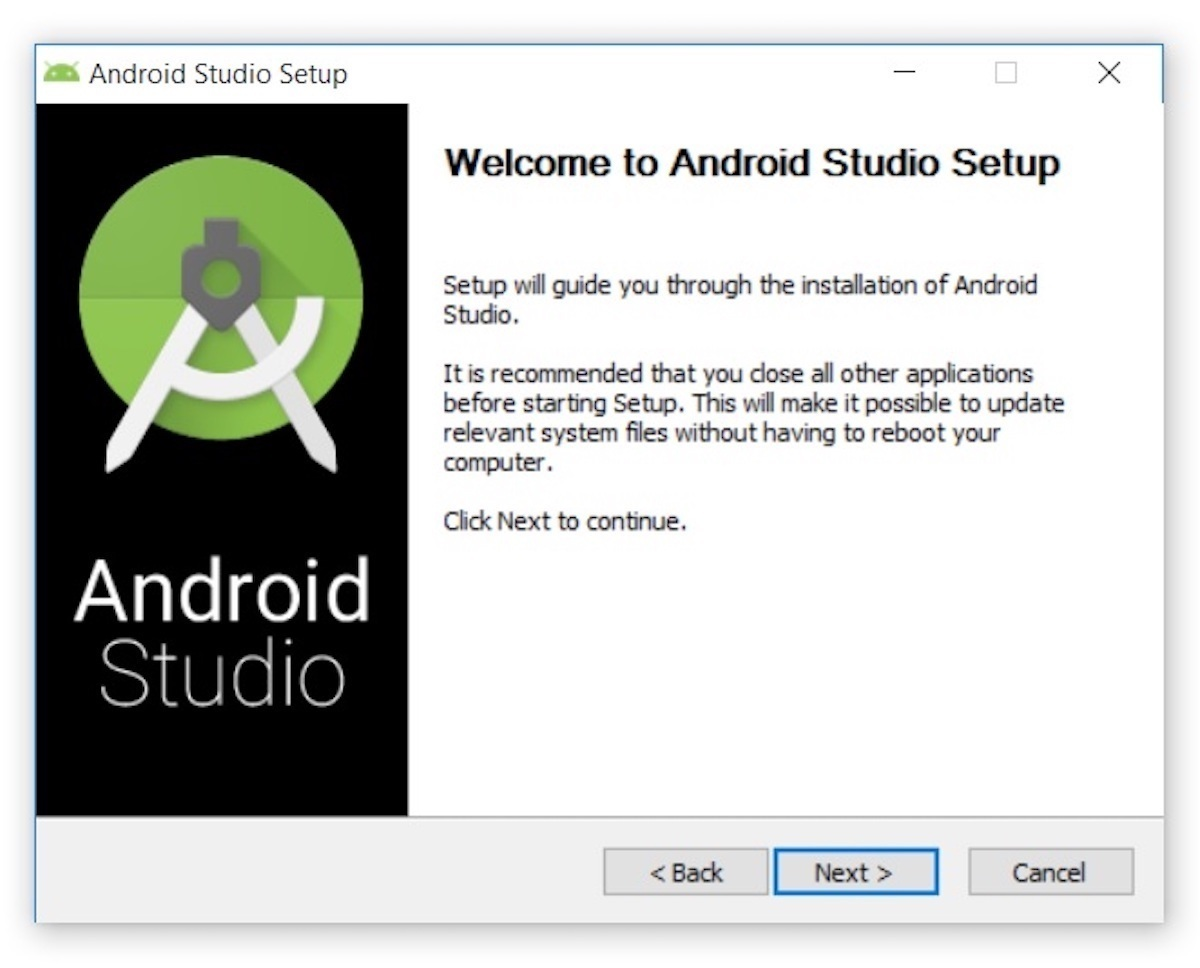
\includegraphics[width=4cm]{figures/installas/1.jpg}
		\centering
		\caption{Android Studio Setup.}
	\end{figure}
	\item Setelah itu kita diberi opsi untuk menginstal Android Virtual Device. Disini kita biarkan default setting-nya, lalu klik Next.
	\begin{figure}[H]
		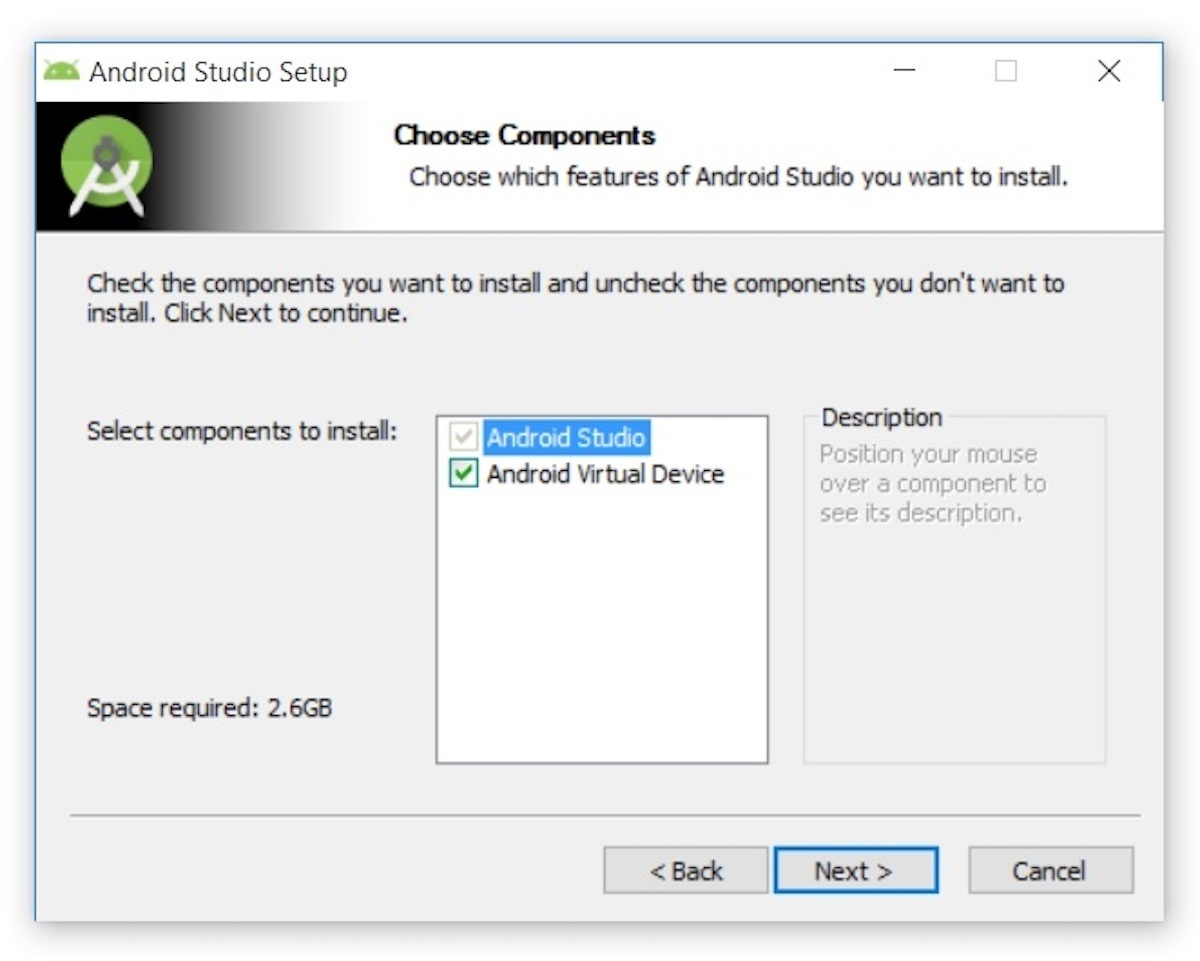
\includegraphics[width=4cm]{figures/installas/2.jpg}
		\centering
		\caption{Instal Android AVD.}
	\end{figure}
	\item Kemudian kita diminta untuk memilih lokasi tempat menginstal Android Studio-nya. Disini kita biarkan default setting-nya, lalu klik Next.
	\begin{figure}[H]
		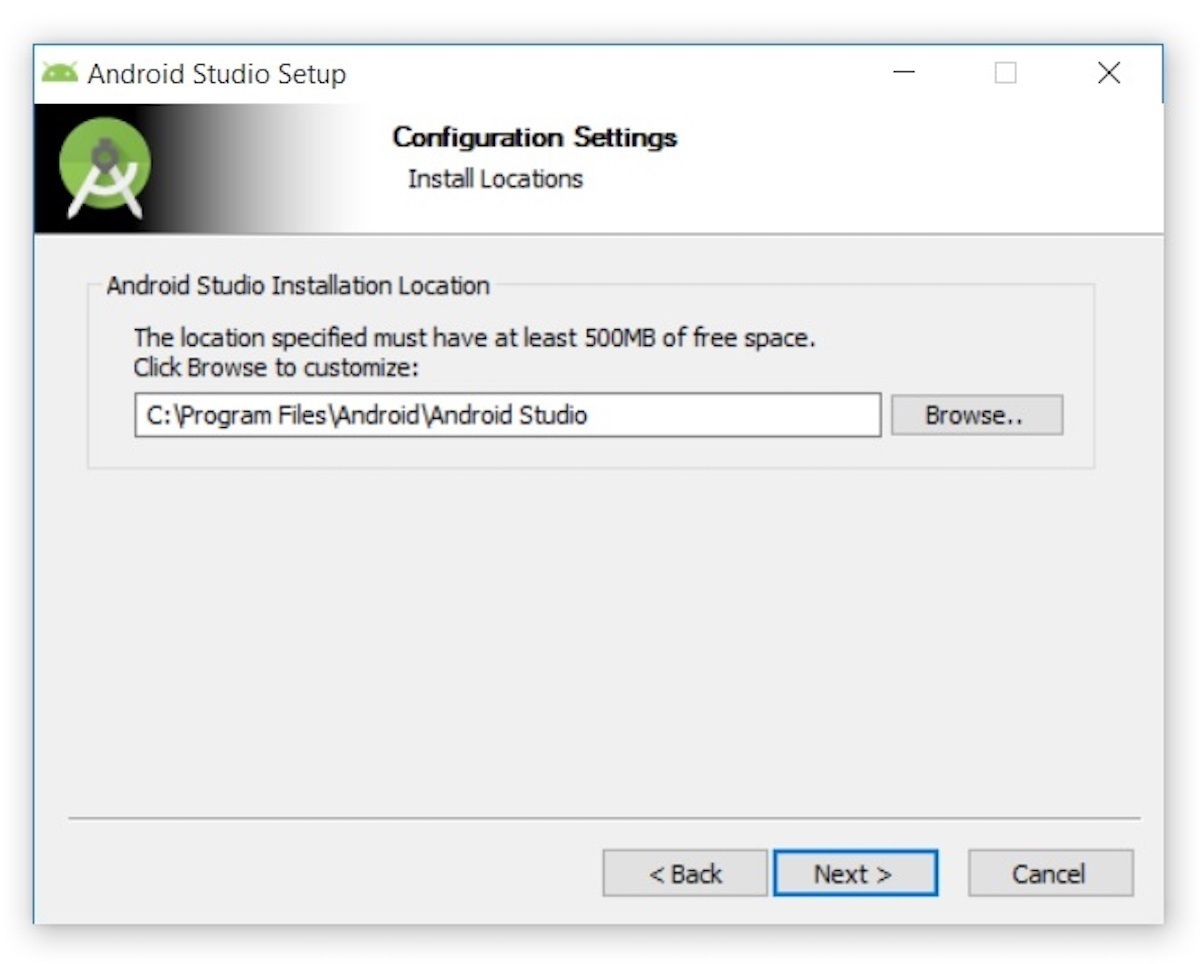
\includegraphics[width=4cm]{figures/installas/3.jpg}
		\centering
		\caption{Lokasi instal Android Studio.}
	\end{figure}
	\item Setelah itu, kita diberi opsi untuk membuat shortcut dari Android Studio. Disini kita biarkan default setting-nya, lalu klik Install.
	\begin{figure}[H]
		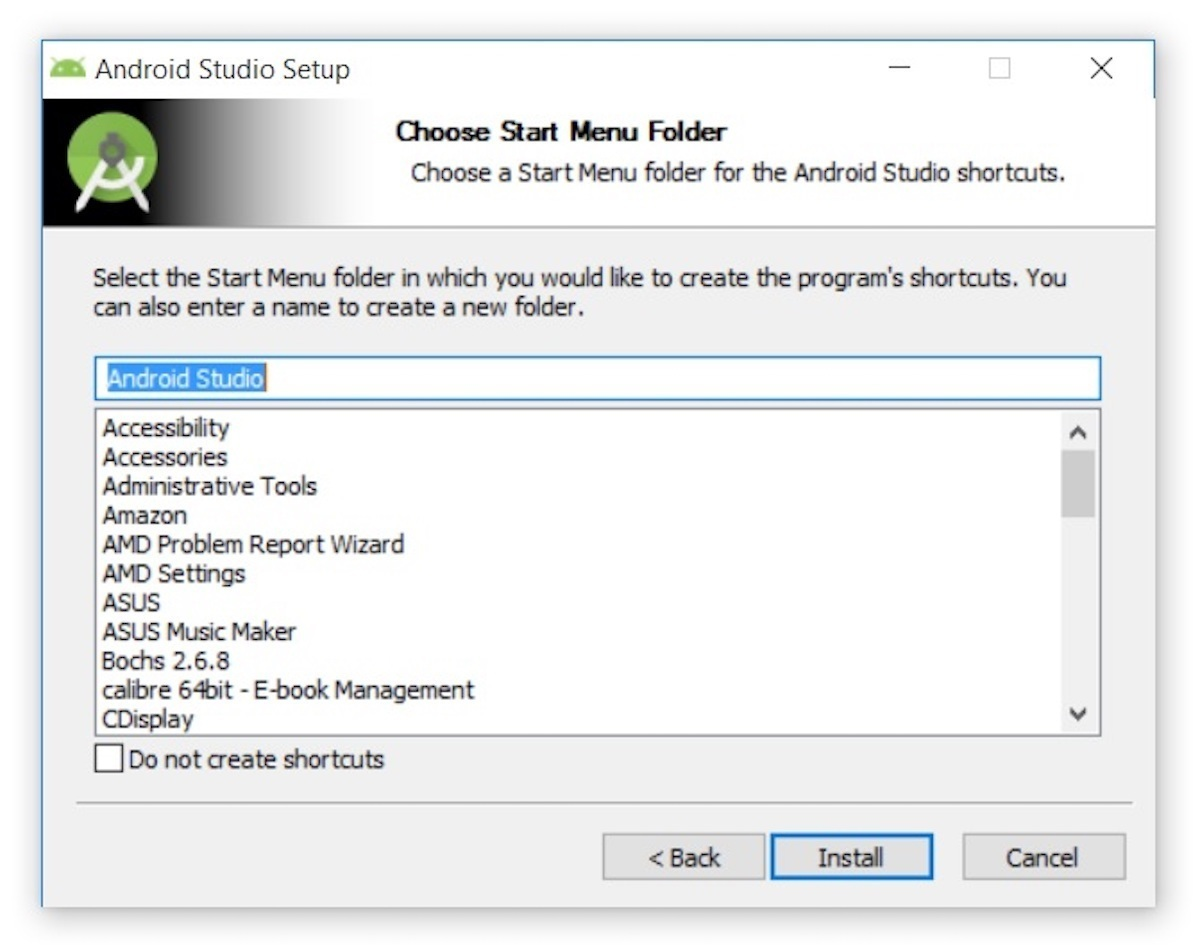
\includegraphics[width=4cm]{figures/installas/4.jpg}
		\centering
		\caption{Membuat shorcut Android Studio.}
	\end{figure}
	\item Kemudian proses instalasi akan berjalan. Show details untuk menampilkan file yang diinstal.
	\begin{figure}[h!]
		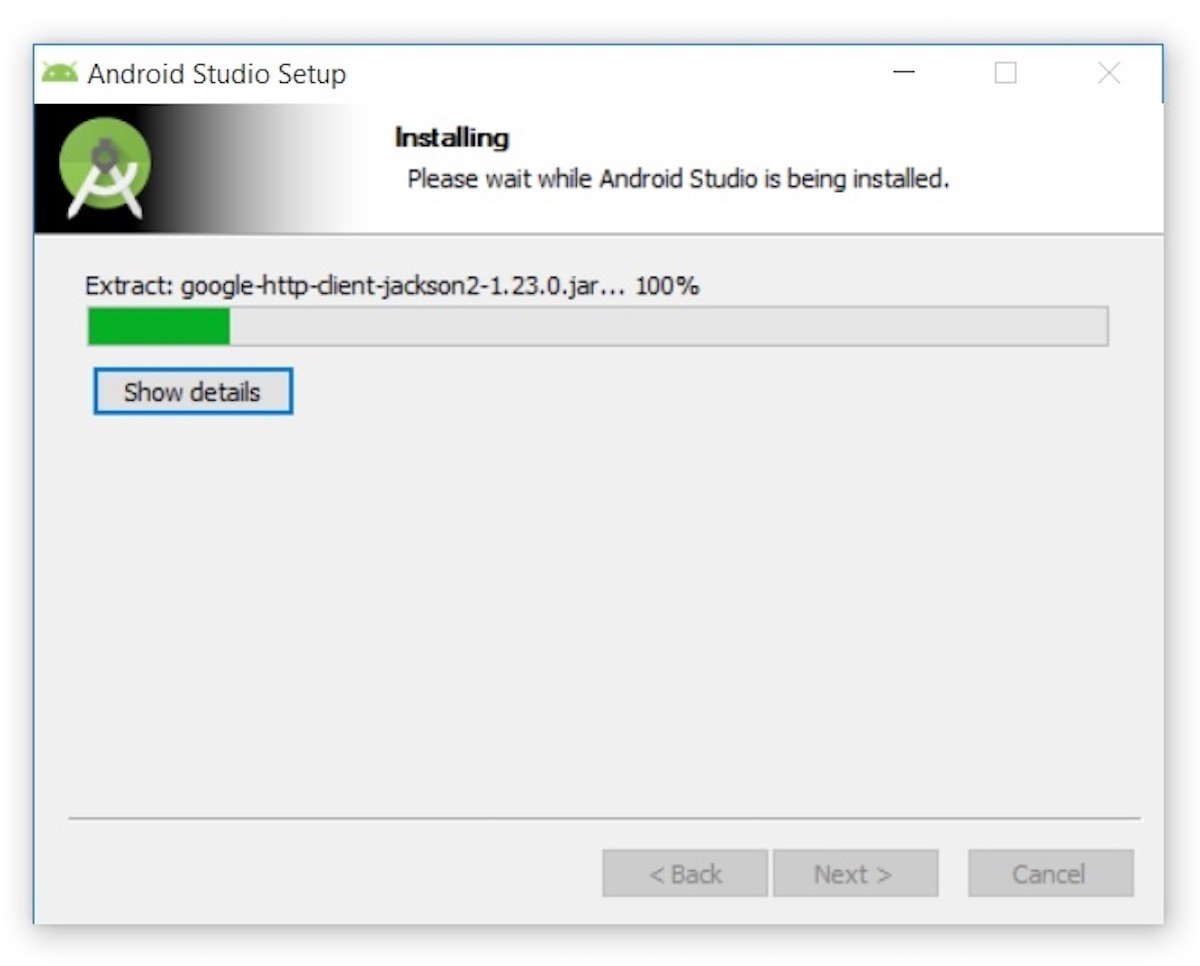
\includegraphics[width=4cm]{figures/installas/5.jpg}
		\centering
		\caption{Proses instalasi.}
	\end{figure}
	\item Setelah proses instal selesai, klik Next.
	\begin{figure}[H]
		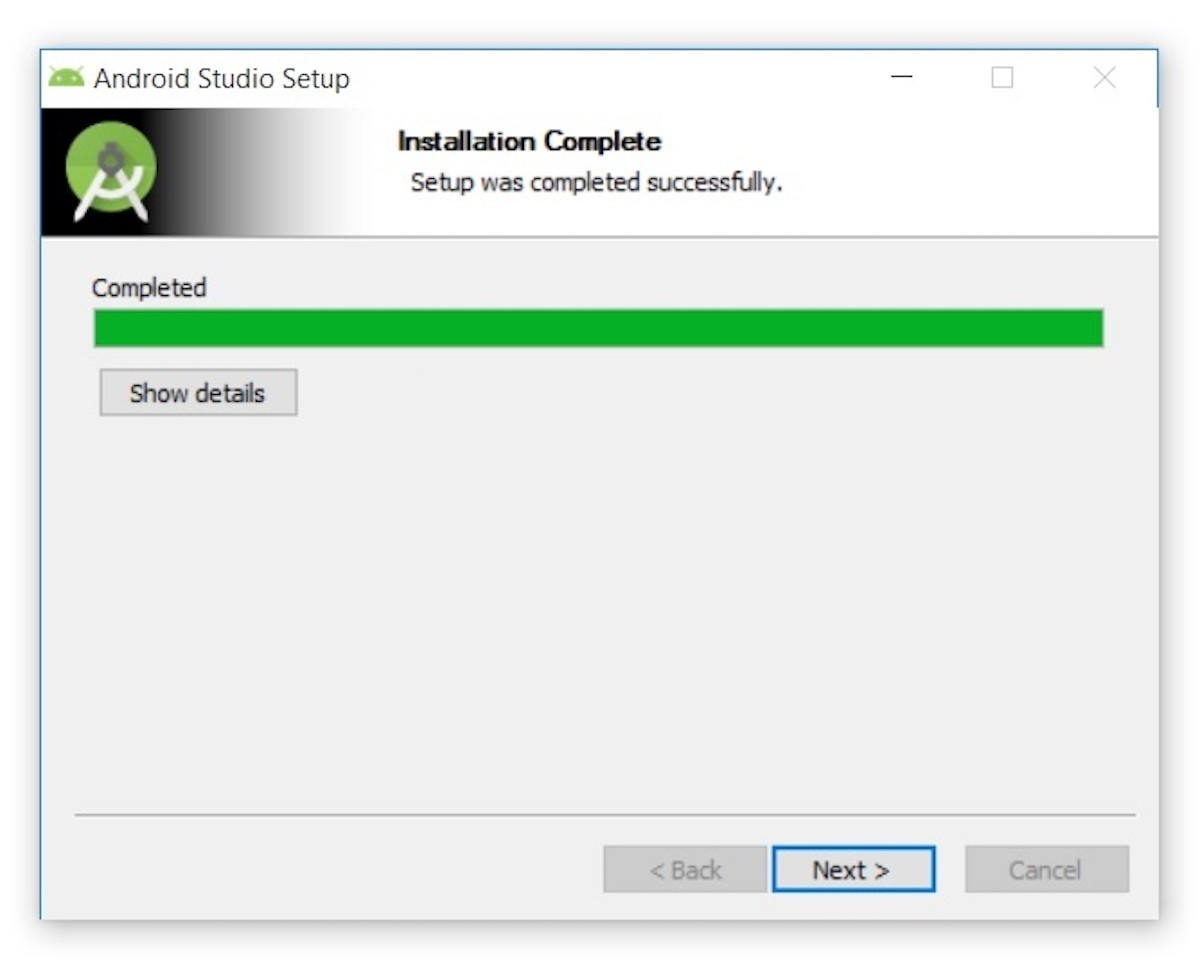
\includegraphics[width=4cm]{figures/installas/6.jpg}
		\centering
		\caption{Proses instalasi selesai.}
	\end{figure}
	\item Kemudian centang Start Android Studio untuk membuka aplikasinya, lalu klik Finish.
	\begin{figure}[H]
		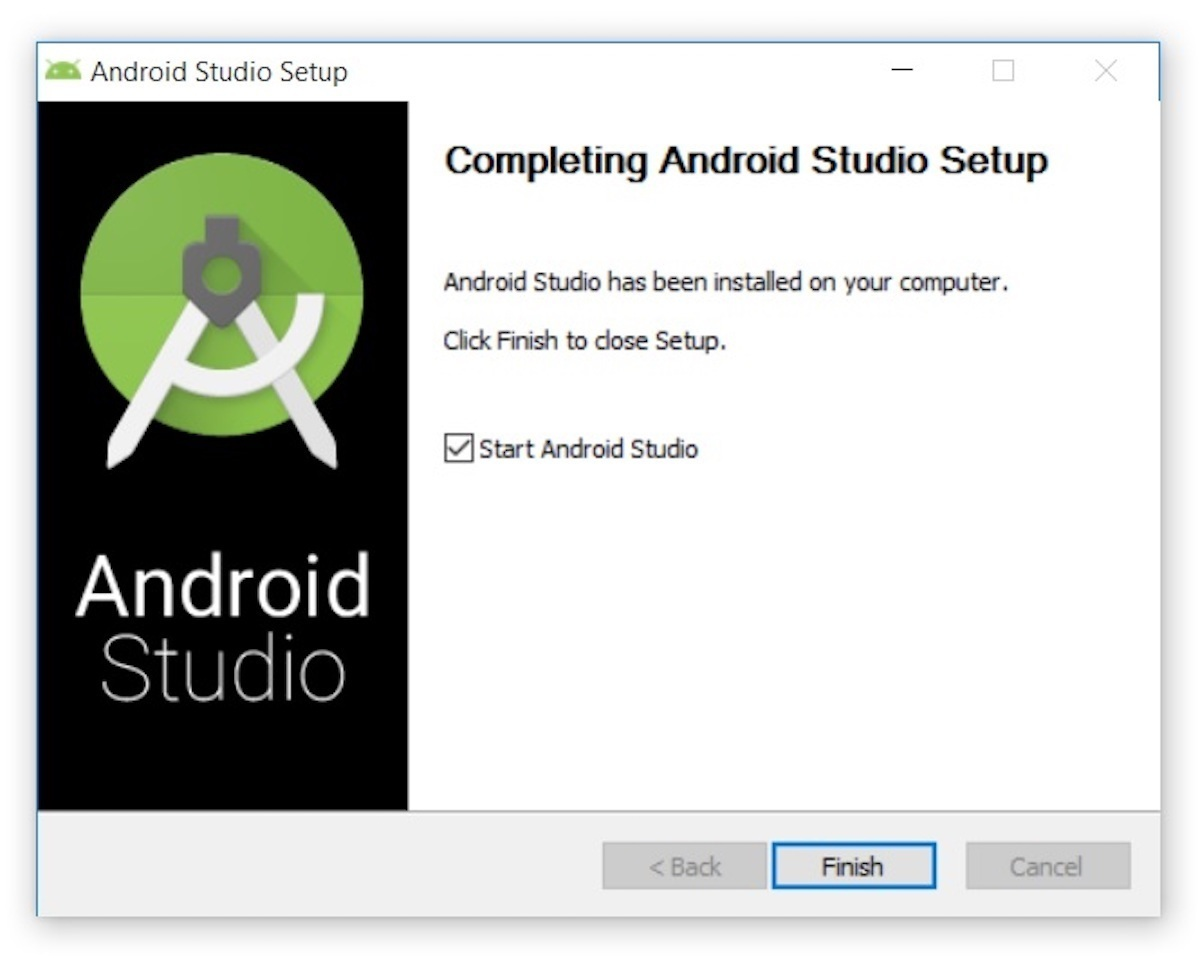
\includegraphics[width=4cm]{figures/installas/7.jpg}
		\centering
		\caption{Jalankan Android Studio.}
	\end{figure}
	\item Ketika Android Studio dijalankan pertama kali, dialog Complete Installation akan muncul dan memberi opsi untuk mengimport setting dari instalasi sebelumnya. Disini kita pilih Do not import settings, lalu klik OK.
	\begin{figure}[H]
		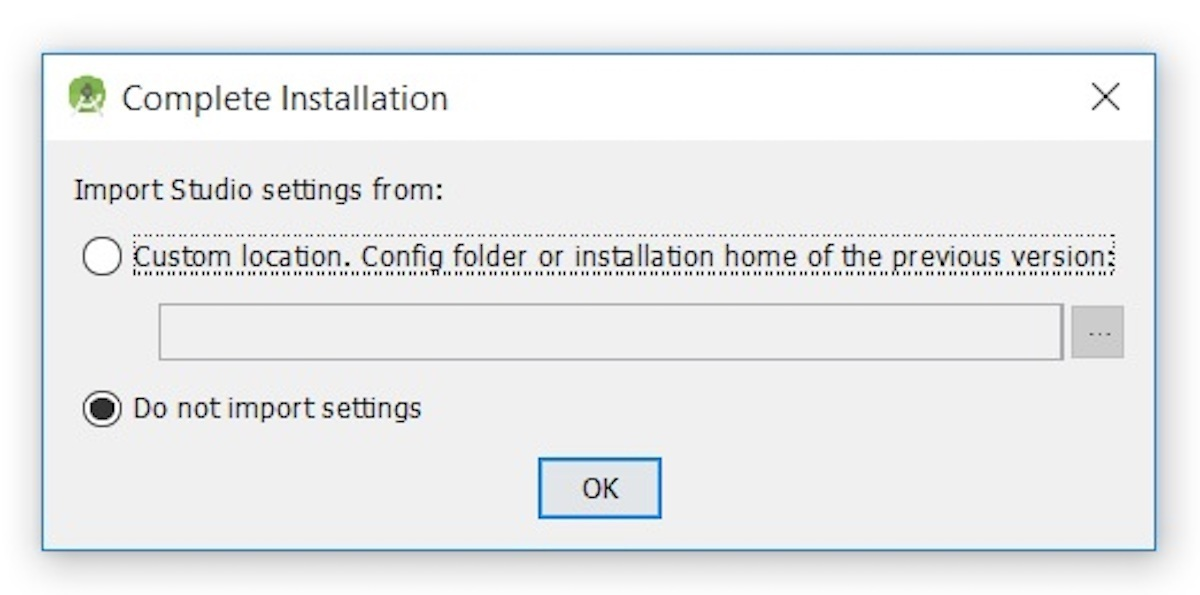
\includegraphics[width=4cm]{figures/installas/8.jpg}
		\centering
		\caption{Import setting instalasi sebelumnya.}
	\end{figure}
	
	\item Kemudian akan muncul splash screen dari Android Studio.
	\begin{figure}[H]
		
\includegraphics[width=4cm]{figures/installas/9.jpg}
		\centering
		\caption{Splash screen Android Studio.}
	\end{figure}
	
	\item Pertama
	\begin{figure}[H]
		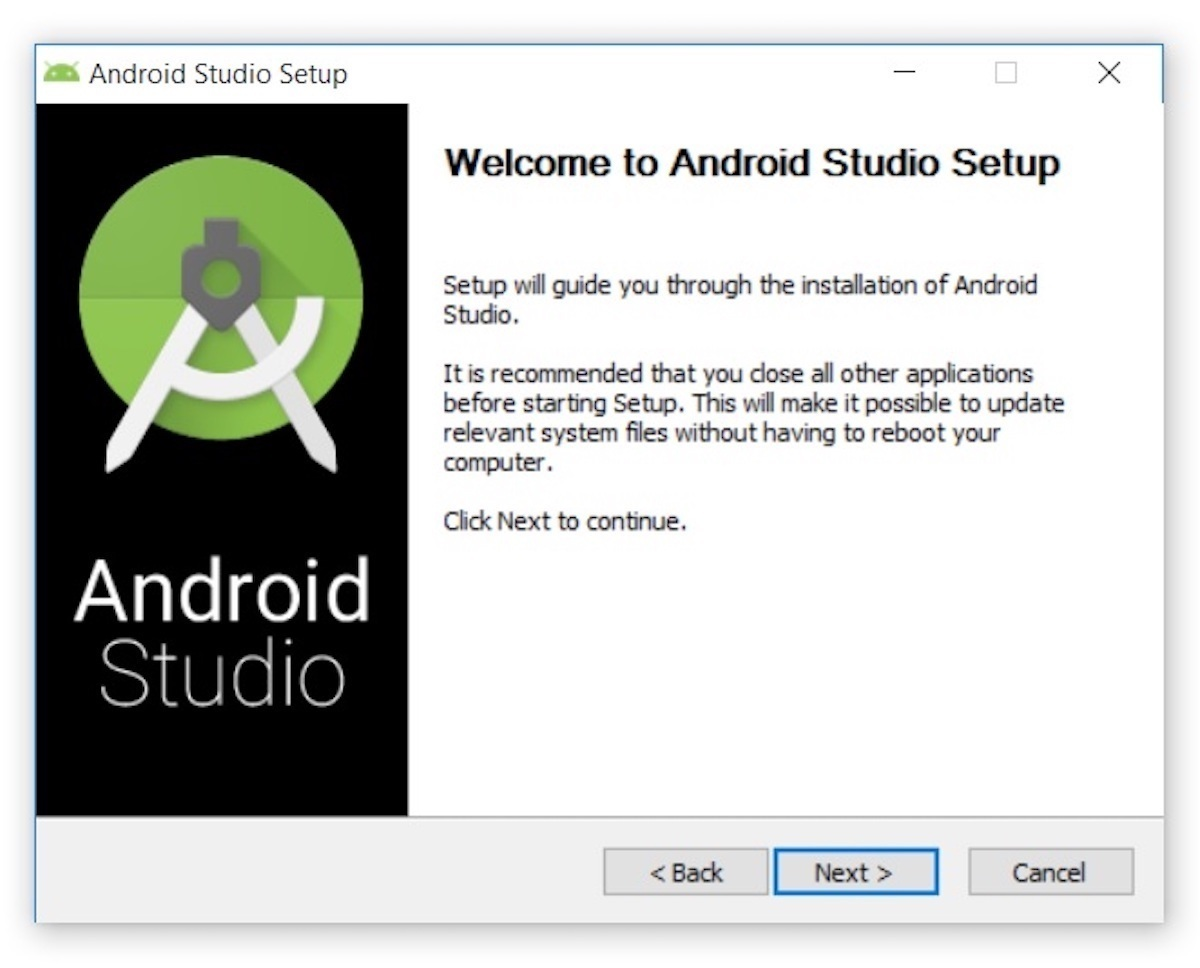
\includegraphics[width=4cm]{figures/installas/1.jpg}
		\centering
		\caption{.}
	\end{figure}
	
	\item Pertama
	\begin{figure}[H]
		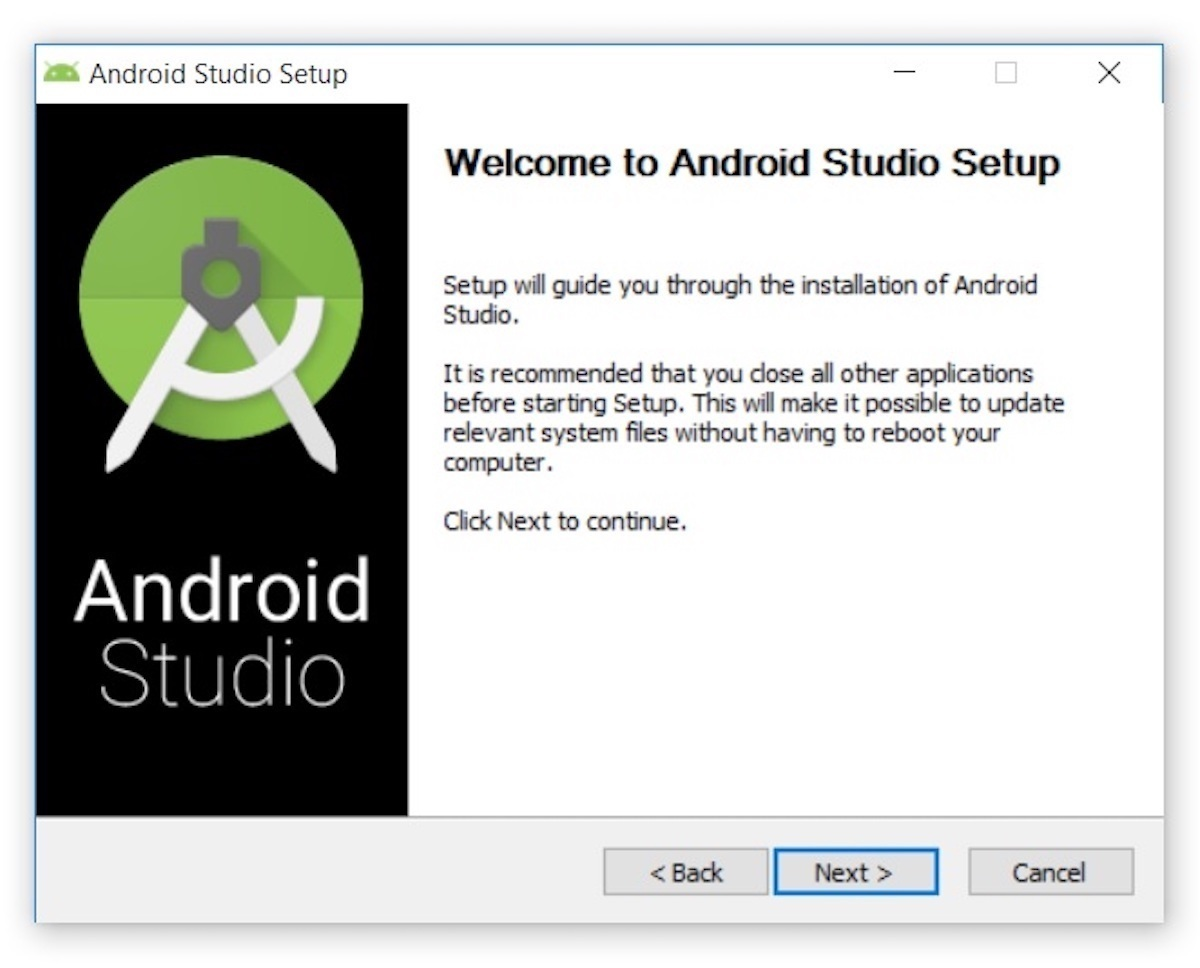
\includegraphics[width=4cm]{figures/installas/1.jpg}
		\centering
		\caption{.}
	\end{figure}
	
	\item Pertama
	\begin{figure}[H]
		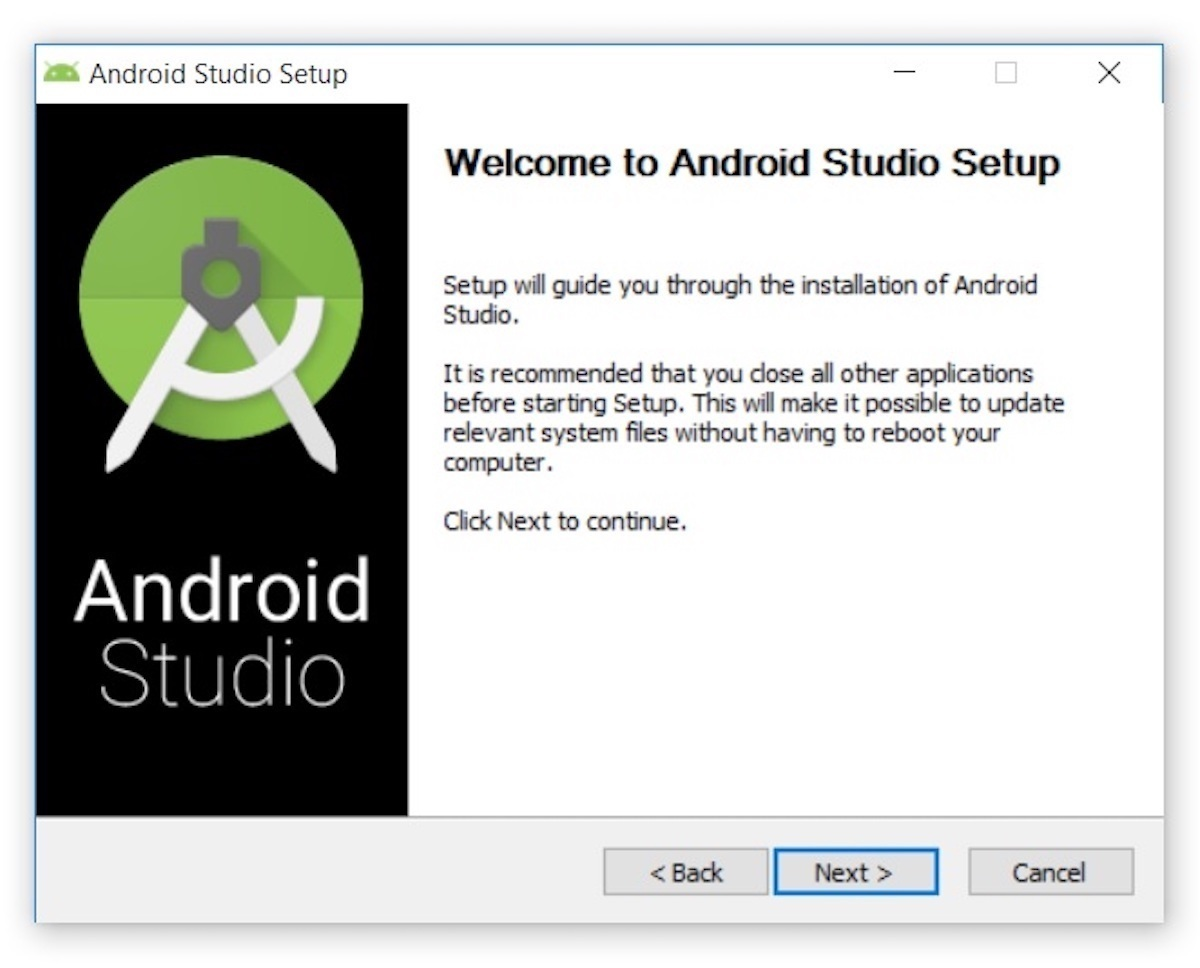
\includegraphics[width=4cm]{figures/installas/1.jpg}
		\centering
		\caption{.}
	\end{figure}
	
	\item Pertama
	\begin{figure}[H]
		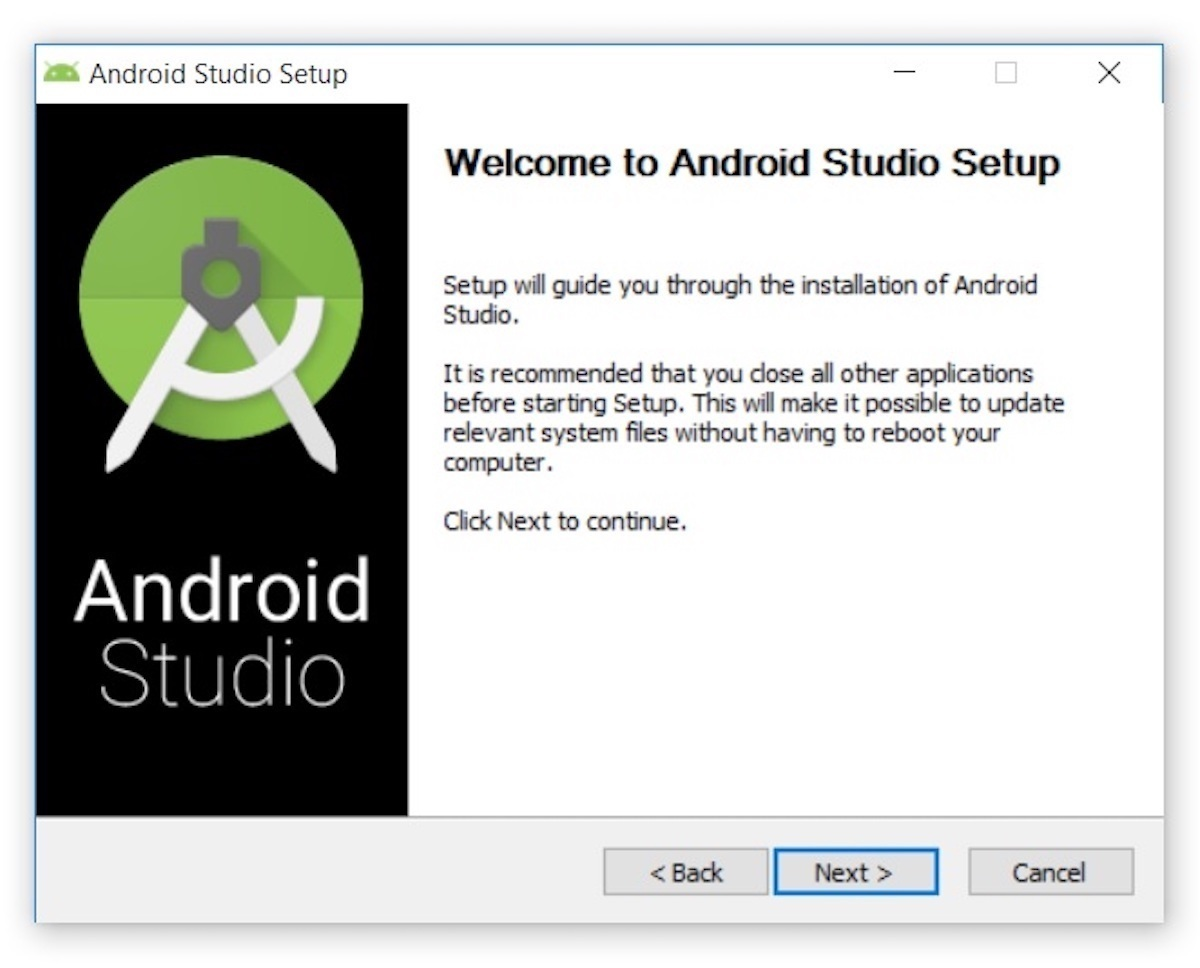
\includegraphics[width=4cm]{figures/installas/1.jpg}
		\centering
		\caption{.}
	\end{figure}
	
	\item Pertama
	\begin{figure}[H]
		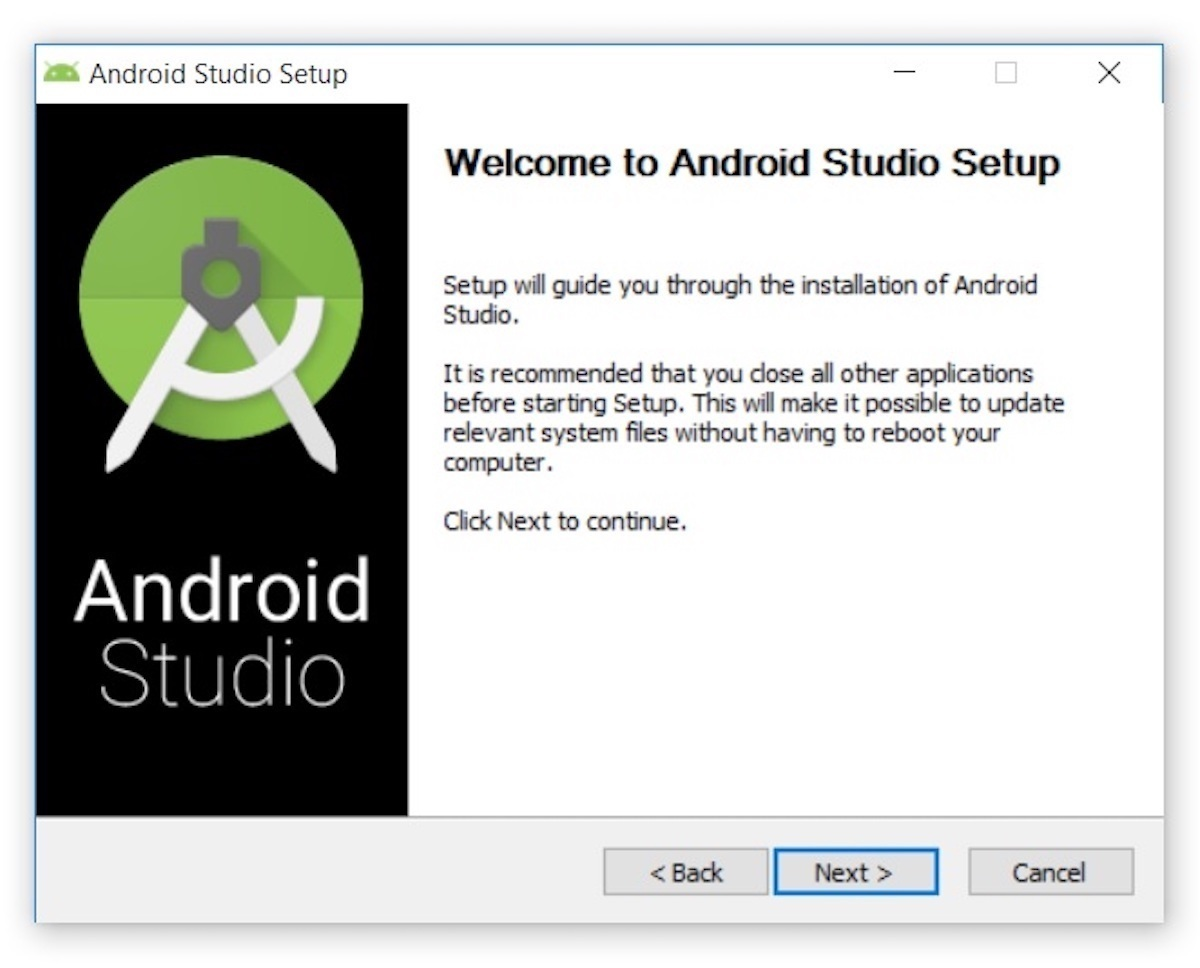
\includegraphics[width=4cm]{figures/installas/1.jpg}
		\centering
		\caption{.}
	\end{figure}
	
	\item Pertama
	\begin{figure}[H]
		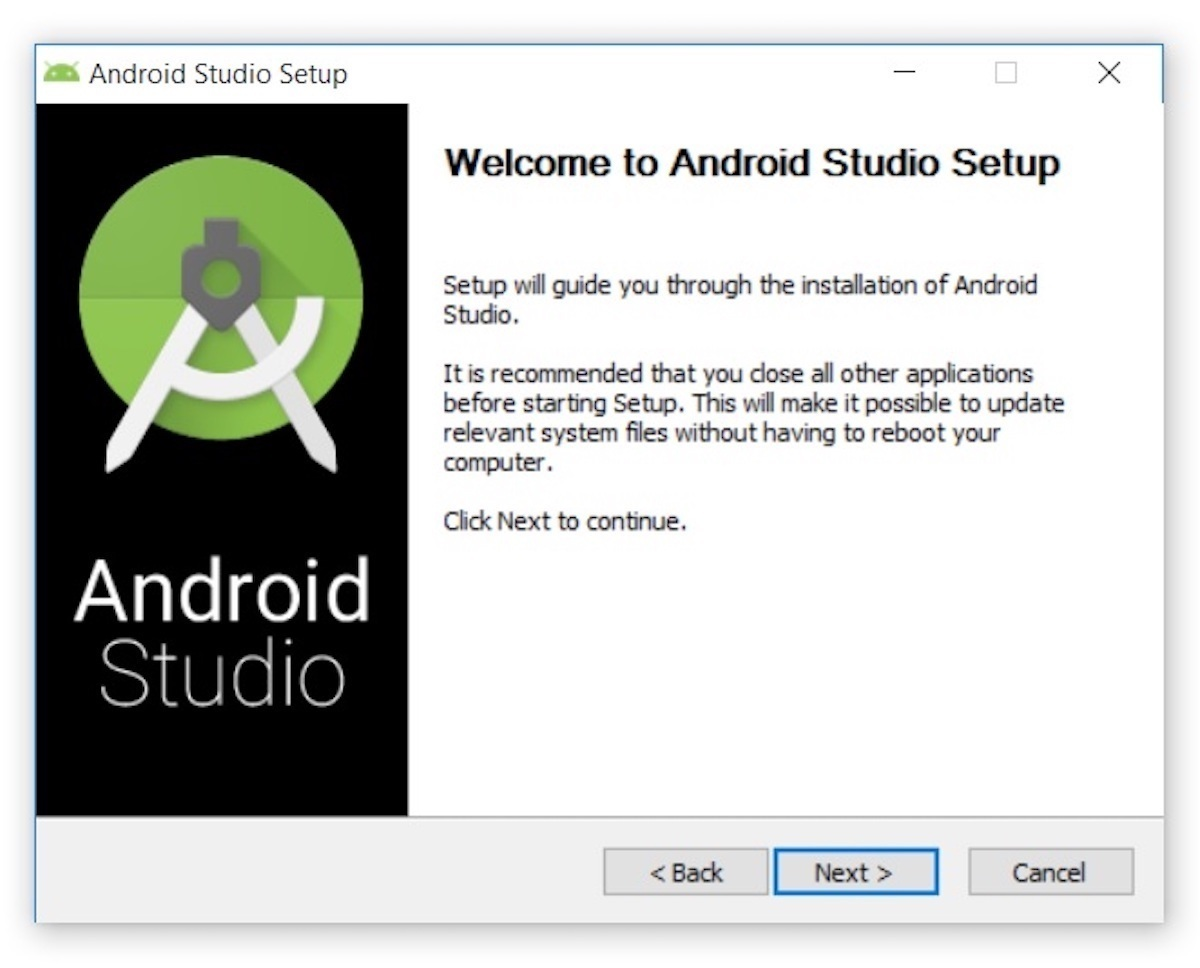
\includegraphics[width=4cm]{figures/installas/1.jpg}
		\centering
		\caption{.}
	\end{figure}
	\begin{figure}[H]
		
\includegraphics[width=6cm]{figures/web/php.png}
		\centering
		\caption{Logo PHP}
	\end{figure}


\subsection{Apa itu PHP?}
PHP merupakan salah satu dari sekian banyak bahasa pemrograman web yang paling umum digunakan dalam pengembangan suatu web. Biasanya dalam implementasinya PHP sering digabungkan atau disisipkan dalam dokumen HTML. PHP memiliki kepanjangan yaitu PHP: Hypertext Preprocessor.Bahasa pemrograman ini bersifat server-side. Arti dari Server-side programming sendiri yaitu script/program tersebut akan dijalankan/diproses oleh server. 

\subsection{Sejarah PHP}
Pada awalnya PHP merupakan kependekan dari Personal Home Page (Situs personal). PHP pertama kali dibuat oleh Rasmus Lerdorf pada tahun 1995. Pada waktu itu PHP masih bernama Form Interpreted (FI), yang wujudnya berupa sekumpulan skrip yang digunakan untuk mengolah data formulir dari web.

Selanjutnya Rasmus merilis kode sumber tersebut untuk umum dan menamakannya PHP/FI. Dengan perilisan kode sumber ini menjadi sumber terbuka, maka banyak pemrogram yang tertarik untuk ikut mengembangkan PHP.

Pada November 1997, dirilis PHP/FI 2.0. Pada rilis ini, interpreter PHP sudah diimplementasikan dalam program C. Dalam rilis ini disertakan juga modul-modul ekstensi yang meningkatkan kemampuan PHP/FI secara signifikan.

Pada tahun 1997, sebuah perusahaan bernama Zend menulis ulang interpreter PHP menjadi lebih bersih, lebih baik, dan lebih cepat. Kemudian pada Juni 1998, perusahaan tersebut merilis interpreter baru untuk PHP dan meresmikan rilis tersebut sebagai PHP 3.0 dan singkatan PHP diubah menjadi akronim berulang PHP: Hypertext Preprocessing.

Pada pertengahan tahun 1999, Zend merilis interpreter PHP baru dan rilis tersebut dikenal dengan PHP 4.0. PHP 4.0 adalah versi PHP yang paling banyak dipakai pada awal abad ke-21. Versi ini banyak dipakai disebabkan kemampuannya untuk membangun aplikasi web kompleks tetapi tetap memiliki kecepatan dan stabilitas yang tinggi.

Pada Juni 2004, Zend merilis PHP 5.0. Dalam versi ini, inti dari interpreter PHP mengalami perubahan besar. Versi ini juga memasukkan model pemrograman berorientasi objek ke dalam PHP untuk menjawab perkembangan bahasa pemrograman ke arah paradigma berorientasi objek. Peladen web bawaan ditambahkan pada versi 5.4 untuk mempermudah pengembang menjalankan kode PHP tanpa menginstal peladen perangkat lunak.

Versi terbaru dan stabil dari bahasa pemograman PHP saat ini adalah versi 7.4.3 yang dirilis pada tanggal 20 Februari 2020

\subsection{Sekilas tentang pembuat PHP : Rasmus Lerdorf}
	\begin{figure}[H]
		
\includegraphics[width=6cm]{figures/web/rasmuslerdorf.jpg}
		\centering
		\caption{Creator PHP Rasmus Lerdorf }
	\end{figure}
Rasmus Lerdorf merupakan seorang programmer yang berasal dari Denmark. Dia membuat dan membantu dalam hal pengkodean bahasa PHP, terutama pada 2 versi awal yang kemudian dikembangkan secara grup bersama dengan Jim Winstead (Yang membuat blo.gs), Stig Bakken, Shane Caraveo, Andi Gutmans, dan juga Zeev Suraski. sampai sekarang ia terus berkontribusi pada projek.

Lerdorf lahir di pulau disko di daerah Greenland dan kemudian pindah ke Denmark pada awal hidupnya. kelaurganya pindah dari Kanada ke Denmark pada tahun 1980, lalu pindah lagi ke kota King di Ontario pada tahun 1983. Dia lulus dari SMA King City pada tahun 1988, dan pada tahun 1993 lulus dari Universitas Waterloo dengan gelar  Bachelor of Applied Science di bidang teknik desain sistem. Dia juga ikut berkontribusi dalam Apache HTTP Server dan menambahkan clausa Limit pada mSQL DBMS. 

Dari Septermber 2002 sampai November 2009, Lerdorf bekerja di perusahaan Yahoo sebagai Infrastructure Architecture Engineer. Pada tahun 2010 kemudian bergabung ke perusahaan WePay untuk mengembangkan API (Application Programming Interface). dan pada tahun 2011 ia menjadi seorang konsultan untuk beberapa startup. Kemudian pada 22 Februari 2012 ia bergabung dengan Etsy, sebuah website e-commerce yang berfokus pada hal hal vintage. Dan pada tahun 2013, Rasmus bergabung dengan Jelastic sebagai Senior Advisor untuk membantu mereka mengembangkan teknologi baru.

Selain itu Lerdorf juga sering menjadi pembicara dalam konferensi open source di berbagai belahan dunia. Beberapa topik yang sering dia bahas diantaranya adalah security vulnerabilities dan juga tentang PHP.

Pada tahun 2003, ia di beri penghargaan oleh MIT Technology Review sebagai salah satu dari 100 inovator di dunia yang berada dibawah umur 35
\subsection{Website yang menggunakan PHP} 
	\begin{figure}[H]
		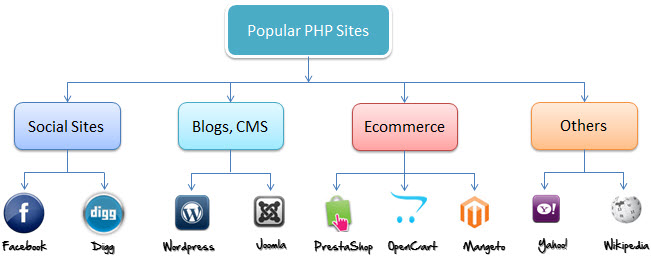
\includegraphics[width=8cm]{figures/web/popularphpsites.jpg}
		\centering
		\caption{Website dengan bahasa PHP}
	\end{figure}

\subsection{Contoh Kode PHP}
	\begin{figure}[H]
		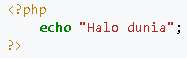
\includegraphics[width=6cm]{figures/web/contohkodingphp.png}
		\centering
		\caption{Program Hello world yang ditulis dengan PHP}
	\end{figure}

\subsection{Kelebihan PHP}
\begin{itemize}
	\item Bahasa Pemrograman PHP dapat ditemukan di mana - mana.
	\item Proses pengembangan lebih mudah, karena komunitas yang bisa dibilang besar dan mendukung.
	\item PHP adalah bahasa scripting yang paling mudah karena memiliki referensi yang banyak dan lengkap.
	\item PHP adalah bahasa open source yang dapat digunakan di berbagai mesin (Linux, Unix, Macintosh, Windows).
	\item Ringkas dan ringan
	\item Maintenanace Mudah
\end{itemize}
\subsection{Kekurangan PHP}
\begin{itemize}
	\item Banyak kompetisi, karena PHP adalah bahasa pemrograman yang paling umum
	\item Terkesan kurang prestigious.
	\item Tidak ideal jika untuk pengembangan skala besar.
	\item PHP mempunyai kelemahan security tertentu.
\end{itemize}

\subsection{Referensi belajar PHP}
\begin{itemize}
	\item php.net
	\item sitepoint.com
	\item tutorialspoint.com/php/
\end{itemize}

	\begin{figure}[H]
		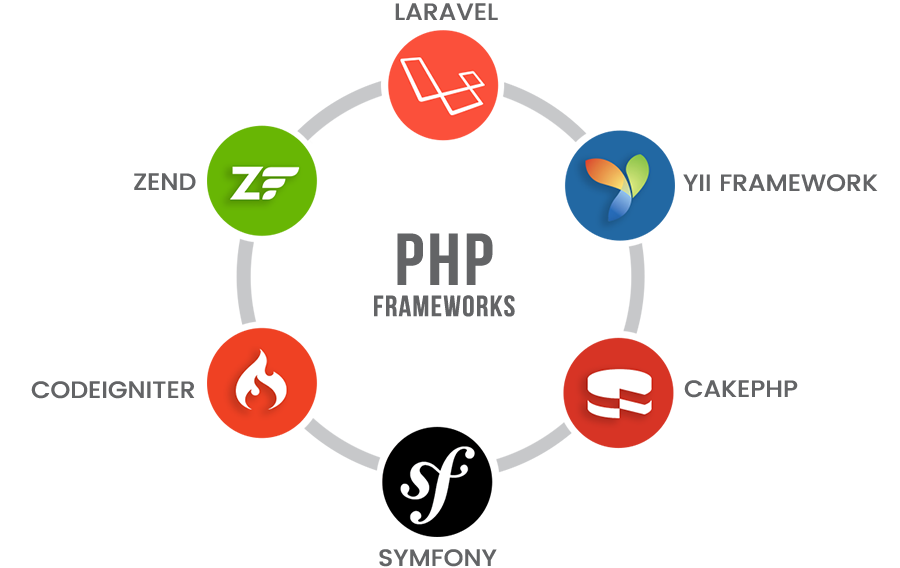
\includegraphics[width=12cm]{figures/web/phpframework.png}
		\centering
		\caption{Framework PHP}
	\end{figure}
\subsection{Apa itu Framework?}
PHP Framework adalah suatu kerangka keja yang telah terbentuk dan tersusun untuk memudahkan proses pengembangan website  secara profesional.

Namun perlu diketahui, bahwa PHP Framework memiliki perbedaannya tersendiri jika dibandingkan dengan sebuah CMS (Content Management System). Meskipun pada dasarnya mereka sama-sama memudahkan dalam hal yang sama yaitu pembuatan website. Tetapi untuk CMS  kita tidak perlu repot-repot dan pusing-pusing menulis script maupun sekumpulan kode. Dengan fitur CMS, semuanya telah dibuat instan dan kita hanya perlu sedikit mengatur bagian konten dan interface-nya saja.

Berbeda dengan Framework, kita tetap harus menuliskan script dan sekumpulan kode untuk dapat membangun sebuah web. 

\subsection{Mengapa harus menggunakan Framework?}
\begin{itemize}
	\item Mempercepat proses pengembangan web
	\item Kode yang terorganisir dan dapat digunakan terus menerus (reusable).
	\item Lebih mudah dalam proses maintenance.
	\item Lebih aman dalam hal sekuriti
	\item Menggunakan pola MVC (model - view - controller) yang memisahkan antara presentation dan logic
	\item Konsep web development modern seperti object oriented programming.

\end{itemize}

	\begin{figure}[H]
		
\includegraphics[width=6cm]{figures/web/logocodeigniter.png}
		\centering
		\caption{Logo Codeigniter}
	\end{figure}

\subsection{Pengenalan Codeigniter}

CodeIgniter sendiri merupakan salah satu framework php yang bersifat aplikasi sumber terbuka(Open Source) dengan model MVC (Model, View, Controller) yang digunakan untuk mengembangkan situs web yang dinamis. CodeIgniter mempermudah proses pengembang web untuk membuat aplikasi web dengan waktu yang lebih cepat dan mudah dibandingkan dengan membuatnya dari awal. CodeIgniter dirilis pertama kali pada 28 Februari 2006. 

	\begin{figure}[H]
		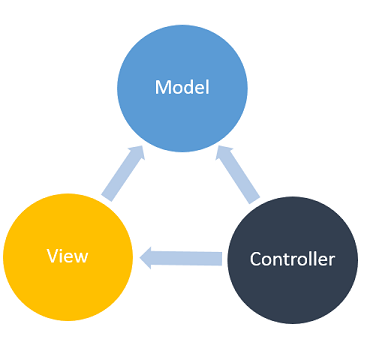
\includegraphics[width=8cm]{figures/web/mvc.png}
		\centering
		\caption{MVC Concept}
	\end{figure}
\subsection{Konsep MVC (Model View dan Controller)}
Model View Controller merupakan suatu konsep yang cukup populer dalam mengembangkan suatu aplikasi web, Konsep MVC ini mencoba memisahkan pengembangan aplikasi berdasarkan komponen-komponen utama dalam membuat suatu aplikasi seperti misalkan bagian untuk pemrosesan/manipulasi data, tampilan , dan bagian untuk kontrol aplikasi. Terdapat 3 jenis komponen yang membangun suatu pola MVC dalam suatu aplikasi yaitu: 
\begin{enumerate}
	\item View, merupakan bagian yang akan ditampilkan dan dilihat oleh pengguna. Biasanya, yang ditampilkan adalah dokumen HTML yang diatur oleh controller. View berfungsi untuk menerima dan merepresentasikan data kepada pengguna. Bagian view tidak dapat memiliki akses pada bagian model.
	\item Model, Berhubungan langsung dengan proses CRUD (Create, Read, Update, Delete), serta search. Model juga menangani validasi dari bagian controller, tetapi berhubungan langsung dengan view.
	\item Controller, merupakan bagian yang menghubungkan model dan juga view, controller berperan dalam menerima data dari view kemudian memprosesnya untuk dikirim ke bagian model.
\end{enumerate}

\subsection{Kelebihan dan Kekurangan Codeigniter}
\begin{itemize}
	\item Kelebihan
\begin{itemize}
	\item Performa sangat cepat.
	\item Konfigurasi yang sangat minim
	\item Komunitas yang aktif dan mendukung
	\item Dokumentasi yang sangat lengkap
\end{itemize}
	\item Kekurangan
\begin{itemize}
	\item CodeIgniter tidak ditujukan untuk pembuatan web dengan skala besar.
	\item Tidak Adanya Editor Khusus.
\end{itemize}
\end{itemize}
\subsection{Instalasi Codeigniter}
\begin{itemize}

	\begin{figure}[H]
		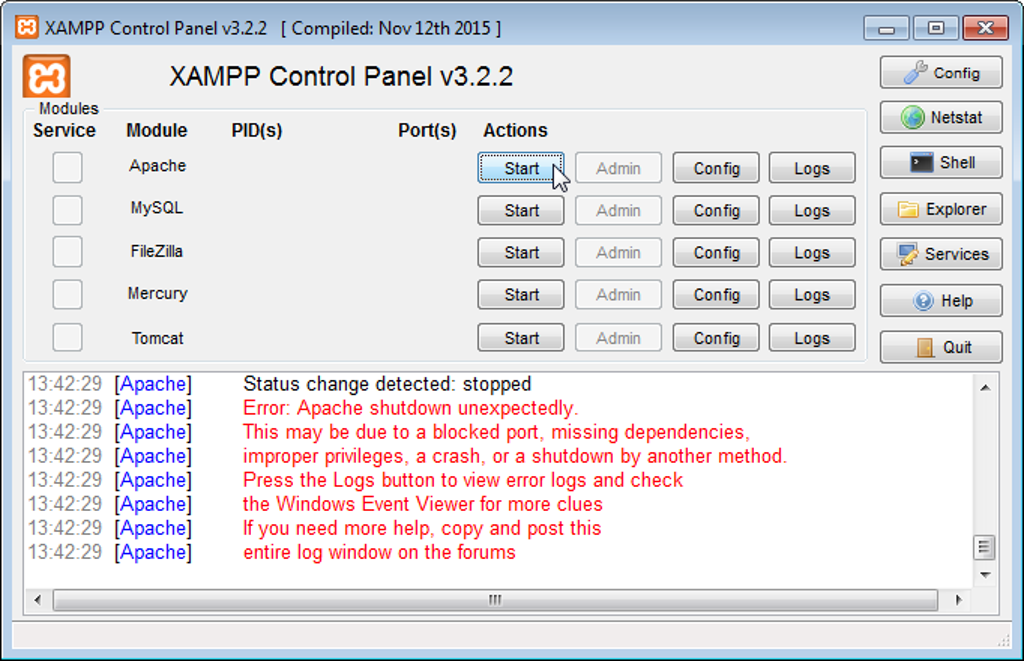
\includegraphics[width=8cm]{figures/web/Xampp.png}
		\centering
		\caption{Tampilan Xampp}
	\end{figure}
	\item Download Xampp terlebih dahulu di https://www.apachefriends.org/
	\item Kemudian install Xampp
	\begin{figure}[H]
		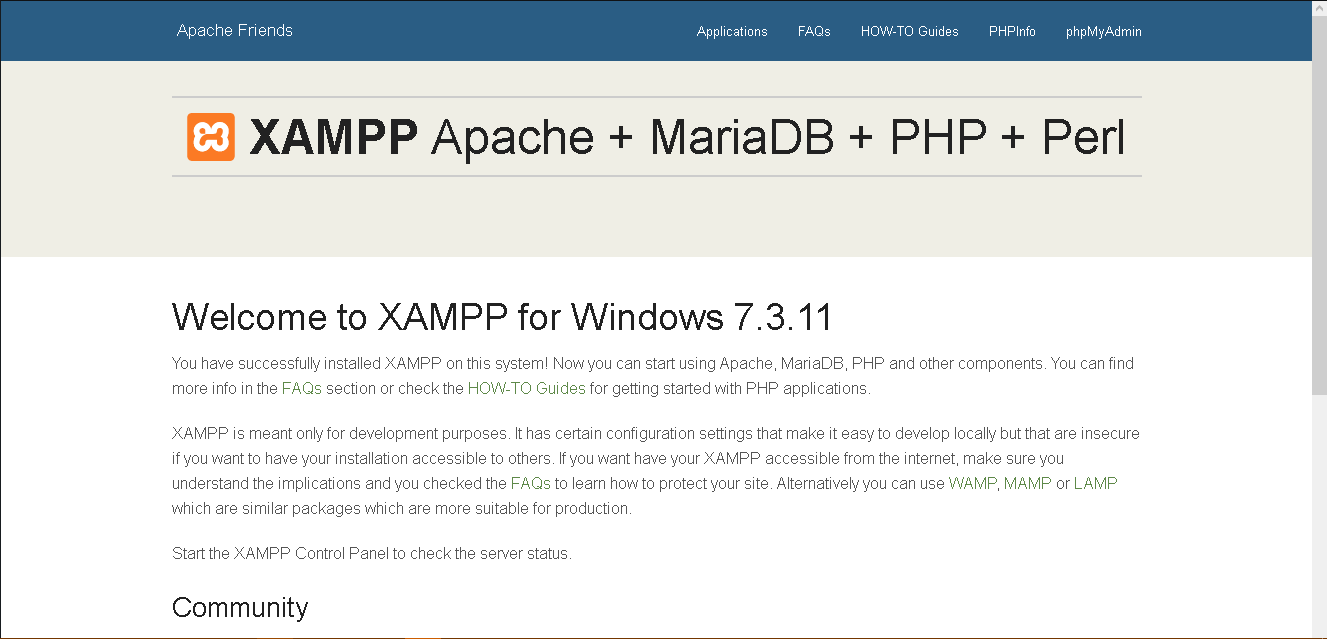
\includegraphics[width=8cm]{figures/web/tampilanwebxampp.png}
		\centering
		\caption{Tampilan web Xampp jika berhasil instalasi}
	\end{figure}


	\begin{figure}[H]
		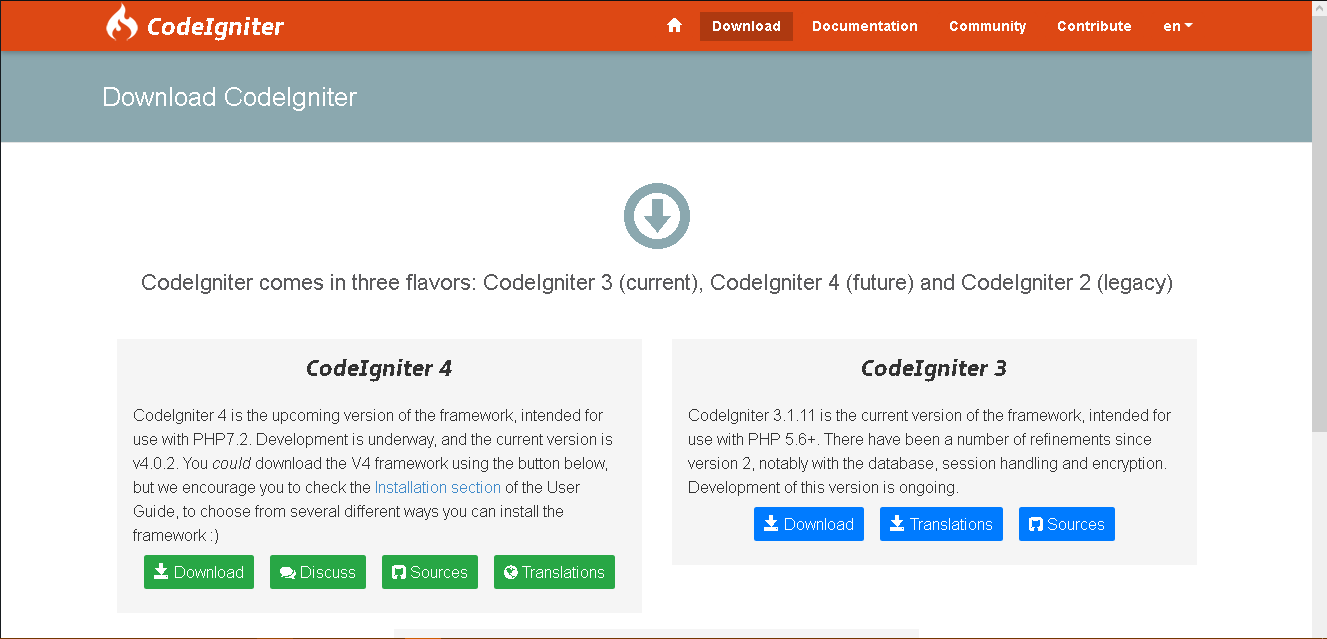
\includegraphics[width=8cm]{figures/web/websitecodeigniter.png}
		\centering
		\caption{Website Codeigniter}
	\end{figure}
	\item Kemudian, dilanjutkan dengan instalasi codeigniter dengan cara mendownload terlebih dahulu codeigniter-nya di https://codeigniter.com/en/download


	\begin{figure}[H]
		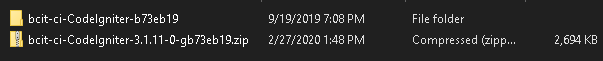
\includegraphics[width=8cm]{figures/web/ekstrakcodeigniter.png}
		\centering
		\caption{Ekstrak File}
	\end{figure}
	\item ekstrak file yang telah di download

	\item berikut adalah hasil ekstrak file
	\begin{figure}[H]
		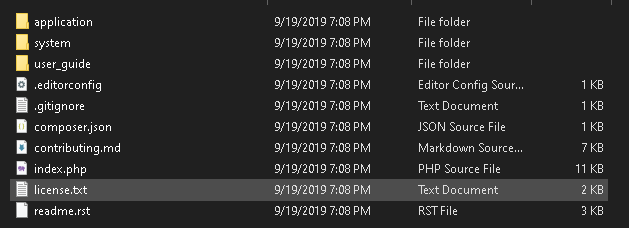
\includegraphics[width=8cm]{figures/web/hasilekstrakcodeigniter.png}
		\centering
		\caption{Hasil Ekstrak File}
	\end{figure}

\end{itemize}

	\begin{figure}[H]
		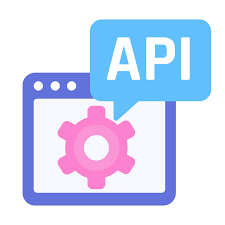
\includegraphics[width=8cm]{figures/GambarAPI.png}
		\centering
		\caption{API}
	\end{figure}
\subsection{Pengenalan API}
API merupakan singkatan yang memiliki kepanjangan yaitu Application Programming Interface, API ini digunakan oleh developer untuk melakukan proses integrasi dua bagian dari satu atau lebeih aplikasi yang berbeda secara bersamaan. API terdiri dari hal-hal seperti function, protocols, dan juga tools. 

Tujuan dari penggunaan API sendiri adalah untuk mempercepat proses pengembangan dari suatu project dengan cara menyediakan beberapa function secara terpisah sehingga para pengembang tidak diperlukan untuk membuat function dengan fungsi tertentu dari awal, langsung pakai saja.

Penerapan API akan memiliki dampak yang signifikan jika fitur yang berkaitan sudah semakin kompleks yang pastinya akan membutuhkan waktu apabila harus memulainya dari awal hanya sekedar untuk membuat function yang memiliki fungsi yang sama dengan API yang telah ada

\subsection{Fungsi API}
API memiliki fungsi untuk menyediakan function yang lebih terstrukur serta terbaca dan mudah dipahami oleh seorang programmer. Hal ini merupakan hal yang krusial, terutama pada bagian editing serta pengembangan suatu projek

\subsection{Jenis-Jenis API}
\begin{itemize}
	\item Ownership Web API
	\item Communication Level API
	\item Web Service API
\end{itemize}
\end{enumerate}



\chapter{Bab 3 : Perancangan}
\section{Perancangan}


\chapter{Bab 4 : Kode dan Implementasi}
\section{Kode dan Implementasi}
Perintah navigasi direktori Android
\lstinputlisting{src/api/config.php}
\lstinputlisting{src/api/conn.php}

\lstinputlisting{src/api/mahasiswa/mahasiswa_login.php}
\lstinputlisting{src/api/mahasiswa/mahasiswa_registrasi.php}
\lstinputlisting{src/api/mahasiswa/mahasiswa_absensi.php}
\lstinputlisting{src/api/mahasiswa/mahasiswa_kegiatan.php}
\lstinputlisting{src/api/mahasiswa/mahasiswa_notifikasi.php}
\lstinputlisting{src/api/mahasiswa/mahasiswa_pembimbing.php}
\lstinputlisting{src/api/mahasiswa/mahasiswa_perusahaan.php}
\lstinputlisting{src/api/mahasiswa/mahasiswa_progress.php}
\lstinputlisting{src/api/mahasiswa/mahasiswa_progress_harian.php}
\lstinputlisting{src/api/mahasiswa/mahasiswa_ubah.php}
\lstinputlisting{src/api/mahasiswa/mahasiswa.php}

\lstinputlisting{src/api/dosen/dosen_login.php}
\lstinputlisting{src/api/dosen/dosen_mahasiswa.php}
\lstinputlisting{src/api/dosen/dosen_notifikasi.php}
\lstinputlisting{src/api/dosen/dosen_progress.php}
\lstinputlisting{src/api/dosen/dosen_progress_harian.php}
\lstinputlisting{src/api/dosen/dosen_ubah.php}
\lstinputlisting{src/api/dosen/dosen.php}

\section{Web}
\subsection{Dapur Hosting}
Di tutorial kali ini kita akan menggunakan jasa web hosting. Web hosting adalah layanan penyimpanan file website, email, dan database yang terkoneksi ke internet dan dapat diakses dengan nama domain. Dapur Hosting menyediakan 2 pilihan lokasi web hosting murah, yaitu di Indonesia dan USA
\begin{itemize}
	\item Siapkan file yang akan di upload
	\begin{enumerate}
\begin{figure}[H]
	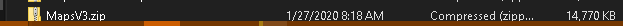
\includegraphics[width=8cm]{figures/web/1_fileupload.PNG}
	\centering
	\caption{Upload.}
\end{figure}	
	\item Login ke dapurhosting
\begin{figure}[H]
	\includegraphics[width=8cm]{figures/web/2_logindapurhosting.PNG}
	\centering
	\caption{Login.}
\end{figure}	

	\item masuk ke file manager dan upload disini
\begin{figure}[H]
	\includegraphics[width=8cm]{figures/web/3_filemanager.PNG}
	\centering
	\caption{Upload file.}
\end{figure}	
	
	\item Setting config database.php
\begin{figure}[H]
	\includegraphics[width=8cm]{figures/web/4_databasesetting.PNG}
	\centering
	\caption{database file.}
\end{figure}	
	\item setting config .php
\begin{figure}[H]
	\includegraphics[width=8cm]{figures/web/5_config.PNG}
	\centering
	\caption{config file.}
\end{figure}	

	\item Hasil
\begin{figure}[H]
	\includegraphics[width=8cm]{figures/web/6_tampilan.PNG}
	\centering
	\caption{Tampilan}
\end{figure}	
	\end{enumerate}
\end{itemize}


Source code web
\lstinputlisting{src/web/config/config.php}
\lstinputlisting{src/web/config/database.php}

\lstinputlisting{src/web/controllers/ckelolauser.php}
\lstinputlisting{src/web/controllers/clogin.php}
\UseRawInputEncoding{src/web/controllers/cregister.php}
\lstinputlisting{src/web/controllers/dashboard.php}

\lstinputlisting{src/web/models/mdatapeta.php}
\lstinputlisting{src/web/models/mdatauser.php}
\lstinputlisting{src/web/models/mlogin.php}
\lstinputlisting{src/web/models/mregister.php}

\lstinputlisting{src/web/views/chartview.php}
\lstinputlisting{src/web/views/dosen.php}
\lstinputlisting{src/web/views/index.php}
\lstinputlisting{src/web/views/login.php}
\lstinputlisting{src/web/views/vgrafik.php}
\lstinputlisting{src/web/views/vkelolauser.php}
\lstinputlisting{src/web/views/vregister.php}








\bibliographystyle{IEEEtran} 
%\def\bibfont{\normalsize}
\bibliography{references}


%%%%%%%%%%%%%%%
%%  The default LaTeX Index
%%  Don't need to add any commands before \begin{document}
\printindex

%%%% Making an index
%% 
%% 1. Make index entries, don't leave any spaces so that they
%% will be sorted correctly.
%% 
%% \index{term}
%% \index{term!subterm}
%% \index{term!subterm!subsubterm}
%% 
%% 2. Run LaTeX several times to produce <filename>.idx
%% 
%% 3. On command line, type  makeindx <filename> which
%% will produce <filename>.ind 
%% 
%% 4. Type \printindex to make the index appear in your book.
%% 
%% 5. If you would like to edit <filename>.ind 
%% you may do so. See docs.pdf for more information.
%% 
%%%%%%%%%%%%%%%%%%%%%%%%%%%%%%

%%%%%%%%%%%%%% Making Multiple Indices %%%%%%%%%%%%%%%%
%% 1. 
%% \usepackage{multind}
%% \makeindex{book}
%% \makeindex{authors}
%% \begin{document}
%% 
%% 2.
%% % add index terms to your book, ie,
%% \index{book}{A term to go to the topic index}
%% \index{authors}{Put this author in the author index}
%% 
%% \index{book}{Cows}
%% \index{book}{Cows!Jersey}
%% \index{book}{Cows!Jersey!Brown}
%% 
%% \index{author}{Douglas Adams}
%% \index{author}{Boethius}
%% \index{author}{Mark Twain}
%% 
%% 3. On command line type 
%% makeindex topic 
%% makeindex authors
%% 
%% 4.
%% this is a Wiley command to make the indices print:
%% \multiprintindex{book}{Topic index}
%% \multiprintindex{authors}{Author index}

\end{document}

